\documentclass{article}
\usepackage[utf8]{inputenc}
\usepackage{hyperref}
\usepackage{float}
\usepackage[table,xcdraw]{xcolor}
%\usepackage[sort&compress,square,comma,authoryear]{natbib}
\usepackage{booktabs}
\usepackage{graphicx}
\graphicspath{{Old_Figures/}}
\usepackage{longtable}
\usepackage{rotating}
\usepackage{geometry}
\usepackage{array}

\usepackage[
backend=biber,
style=authoryear,
sorting=nyt % sort by name year title
]{biblatex}
\addbibresource{Ref_invertebrate_DB.bib}

\title{ DRAFT: Harmonized macroinvertebrate trait database, Aggregation of traits, Trait definitions }
\author{}%Stefan Kunz 
\date{}%June 2019


\begin{document}
%TODO: Use citep & citet instead of cite
\maketitle

\section{Introduction}
% Half of all described freshwater invertebrates are aquatic insects
% In the age of the Anthropocene invertebrates are exposed to multiple stressors such as chemical pollution, hydro-morphological modifications, invasive species and climate change. %?Sources 
% Freshwater invertebrates play a crucial role for many ecosystem processes such as carbon cycling and water purification. In addition to their functional role,
% Ten \% of all described species live in freshwaters, most of them being invertebrates, and thus represent a large part of animal biodiversity.

%! Understanding species distributions
Understanding distributions of invertebrate communities and predicting effects of potential natural or anthropogenic stressors is a long time goal of freshwater research. Since the 1970s ecologists have started using organismal characteristics or traits to group aquatic insect species to understand their diversity. The first to do so was Cummins by assigning feeding mechanisms to aquatic insects (\cite{cummins_trophic_1973}). Since then many studies have been carried out trying to use invertebrate traits to understand ecosystem processes, as tool for biomonitoring, and the effects of multiple stressors on freshwater communities (\cite{statzner_can_2010, menezes_beyond_2010}). 
% TODO: needs further citation
As a result, comprehensive databases on freshwater invertebrate traits have been compiled over the years (see table \ref{tab:trait_databases} for examples).

Traits are defined as measurable characteristics and ecological preferences at the individual organism. %TODO: add citation
They reflect an organisms adaptation to its habitat and provide a mechanistic link between a species and its environment. Trait based approaches in ecology have its theoretical foundation in the habitat template theory, that predicts where environmental conditions are similar trait composition should also converge, even across biogeographic boundaries (\cite{southwood_habitat_1977}). %TODO: cite Poff
Several studies suggested that trait variability is lesser on larger geographical scales than taxonomic variability (\cite{bonada_taxonomic_2007}). Therefore, trait based approaches can be a suitable tool for comparing the effect of various environmental stressors to invertebrate communities on large scales or across regions. 
%? Source: Statzner & Beche 2010, Ralf Paper
Consequently, studies have been carried that e.g. examine the relationship between climate change and freshwater community assemblages using species traits (\cite{bhowmik_large_2015, brown_functional_2018}).
% More citations
% ? Enrich with examples -> Maybe for toxicants as well?
Many of such studies combine information from several trait databases. For example, Brown et al. used invertebrate trait databases from Europe, North America and New Zealand to investigate the effect of decreasing glacier cover to river ecosystems (\cite{brown_functional_2018}).
% Studies that use information on aquatic invertebrate traits from different regions
% and/or aggregate trait information are increasing 
% !Transition into trait data
As mentioned earlier, invertebrate trait data have become increasingly available over the last decades, also for different regions.

% !Mention various problems with trait databases 
However, researchers face various problems when they need to synthesize information from multiple invertebrate trait databases. 
% !Trait terminology
I) The use of inconsistent terminology across studies (see \cite{schmera_proposed_2015} for a comprehensive discussion). 
For example, some studies used the term \textit{trait} to describe a general organismal property like "generations per year" (\cite{statzner_reproductive_1997}, \cite{ussegliopolatera_biological_2000}), while in other studies this 
term was related to categories like "bi/multivoltine" (\cite{haybach_use_2004}, \cite{vieira_database_nodate}). Here, we follow 
the proposal of Schmera et al. (2015) and use the term \textit{trait} for a morphological, physiological, or phenomenological feature measurable at the individual organism (e.g. tegument, gills, etc.) and the term \textit{grouping feature} to describe a general property of related organismal traits (e.g. respiration). The \textit{membership state} gives the measurement scale (normally nominal or ratio scale) the trait is described on.
%! Different traits used/definitions
II) Invertebrate trait databases from different regions are not standardized. Often, the same grouping features are categorized using different traits. 
% TODO Example
This is complicated by the use of different measurement scales. For example, trait databases from North America use traditionally a binary coding (i.e. trait is expressed or not), whereas most other trait databases (e.g. Tachet, freshwaterecology, and New Zealand) use fuzzy coding (i.e. trait is expressed to a certain extent by the organism). Hence, transformation of nominal scale to ratio scale or vice versa is required. %? Wording
Furthermore, definitions and terminology applied to traits differ as well across databases. Recently, Schneider et al. advocated standard terminologies and ontologies for trait definitions after finding that trait databases for different organism groups (inter alia invertebrates) are rarely standardized and have low potential for data synthesis (\cite{schneider_towards_2019}).
% ?Example (feeding)
%! Taxonomical resolution & traits aggregation -> no guidance
%! Wording: taxonomical resolution -> high -> species level 
% high taxonomical level -> high -> genus/family,...(Schmidt-Kloiber et al.)
III) Taxonomical resolution between databases differs, further complicating the synthesis of trait data from multiple regions. Some trait databases have recorded information on mixed levels of taxonomical resolution like the North American trait database or the Australian trait database. In contrast, trait information in the freshwaterecology database is entirely recorded on species-level. %?ref to graphic
%TODO: Percentages of different levels of taxonomical resolutions in process overview graph 
Using trait information on varying taxonomical levels is only possible when traits are aggregated to the lowest taxonomical level that is shared by all used databases. However, IV) so far studies comparing different ways of aggregating traits are lacking.
% Hence, guidance on how to perform a robust trait aggregation is missing. 
% TODO Poff Paper example, check Brown and other literature

%!Incentive of our analysis:
Given the problems mentioned above extensive data processing is required before researchers can use multiple invertebrate trait databases for their work. In this paper we examine difficulties that ecologists face when synthesizing trait information from multiple databases. We explore the effect of different decisions researches have to make when working with invertebrate trait data from several sources, involving trait harmonization, handling different codings, normalization, and aggregation of traits.
%?Effect of a statistical analysis -> Clustering?
%!What we did/Goal:
Therefore, we harmonized six grouping features of different macroinvertebrate trait databases from four regions and aggregated the trait information to family-level. % ?Name Traits
We discuss the harmonization and show the effect of different ways of aggregating traits. We also present an overview of differences in trait definitions among databases. Finally, our paper compares the references for the trait information that were specified in the trait databases we used.

%TODO: Change heading to be more expressive
\section{Methods}

\subsection{Description of harmonized trait databases} 

% TODO Give a motivation (better in introduction?)
The harmonized databases are using the available information on aquatic invertebrate traits for the regions Europe, North America, Australia, and New Zealand. Due to the different number and identity of grouping features in each database, the following six grouping features were chosen for this study: locomotion, feeding mode, respiration, voltinism, size, and body form. 
% TODO: Few words why these grouping features have been selected
% TODO: Reasoning why no ecological grouping features have been used
Trait information for Australia and New Zealand were retrieved from a single database, respectively. For Europe we gathered trait information from the freshwaterecology trait database (\url{https://www.freshwaterecology.info/}) and complemented where possible missing information with the 
Tachet trait database (\cite{usseglio-polatera_biomonitoring_2000}). North American invertebrate traits were retrieved from Laura Twardochleb and 
complemented where possible by trait information from Vieira et al (\cite{vieira_database_nodate}). From now on, if we use the term European or North American trait database we refer to the combined databases. We used all available information on invertebrates in the databases but restricted our analysis to those taxa that have complete trait profiles for the investigated grouping features. We are aware that imputation methods exist, which infer missing information for traits by interpolating from related traits (\cite{penone_imputation_2014}). However, by using only complete data we were able to evaluate the taxonomical coverage within the databases. We consider this a helpful information for researchers who strive to fill data gaps. Table \ref{tab:trait_databases} gives an overview of the used databases. 
% In the following paragraphs, we describe the data processing steps required to establish a harmonized invertebrate trait database. The results section trait aggregation methods are compared with each other and with traits assigned at family-level
% The rest of the paper is structured as following:
 % Trait definitions are compared and discussed in chapter...
\begin{table}[H]
    \centering
    \caption{Overview of trait databases.}
    \label{tab:trait_databases}
    \begin{tabular}{lll}
    \toprule
   Region & Coding of trait states & Reference \\ 
    \hline
   Europe & Largely fuzzy & \cite{schmidt-kloiber_www.freshwaterecology.info_2015}\\ 
   Central Europe & Fuzzy coded & \cite{usseglio-polatera_biomonitoring_2000} \\ 
   North America & Largely binary & \cite{vieira_database_nodate}\\
   North America & Largely binary & cite Laura Twardochleb \\
   Australia & Binary \& fuzzy coding  & \cite{kefford_ben_AST_DB_2019}\\ 
   New Zealand & Fuzzy coded & \\ %TODO: Create entry for more recent NZ reference
    \bottomrule
    \end{tabular}
\end{table}


\subsection{Normalization \& data conversion}

%TODO Mention taxonomical corrections?
% !Issues with coding & scale in the trait databases
Establishing a harmonized database required traits on the same measurement scale to enable comparability. However, in the used databases traits varied within and among databases in terms of measurement scale. Traits were either fuzzy coded, binary coded or to a small extent coded as continuous variable (e.g. size). Fuzzy codes capture the variation (i.e. temporal or spatial) in a trait and are represented by affinity scores which express the preference of a taxon to a certain trait. Usually, these scores range from 0 representing no affinity to an arbitrary maximum value which represents high affinity. This type of coding uses the ratio scale and not the ordinal scale. In fact, the intention of the developers of this coding system was to convert affinity scores to percentages per trait, e.g. for a grouping feature with four traits affinity scores of \textit{5, 6, 2, 2} are equal to \textit{1/3, 2/5, 2/15, 2/15} or \textit{33.3 \%, 40 \%, 13.3 \%, 13.3 \%} (\cite{chevenet_francois_fuzzy_1994}). We used fuzzy coded traits for establishing our harmonized databases where possible, otherwise binary traits. Categorical and continuous traits across all used databases were converted into binary traits. Implicitly, we assumed for binary variables that a value of 1 for a particular trait corresponded to the maximum affinity of a taxon for that particular trait.

Two databases needed further data processing. Firstly, the Australian database which is a collection of seven trait databases. Thus, several grouping features occur multiple times but with traits that have different types of codings and ranges. For example, body size occurs as continuous variable, with traits that are fuzzy coded, and with traits that are binary coded. The same traits originating from different sub-databases in the Australian trait database were allocated. To enable allocation of fuzzy coded and binary traits we applied a range normalization by dividing each fuzzy coded trait by its potential maximum value. Consequently, the values of each trait were converted to a range from 0 to 1.

Secondly, the North American trait database which only contained traits on the nominal scale. We first converted nominal traits into binary traits. As a second approach we converted nominal traits for taxa on species and genus-level into "pseudo" fuzzy codes by calculating the percentage of occurrence for each trait per genera and grouping feature. Both approaches were compared regarding the trait values they yielded.
% We refer to the version with binary traits as \textit{NOA\_bin} and to the version with pseudo fuzzy codes as \textit{NOA\_fuzzy}.
% Better wording? traits from NOA data were converted to fuzzy codes by allocating at genus level using frequency on species level

% Furthermore, in some databases fuzzy coded information occurred in different ranges 
% (e.g. from 0 to 3 and from 0 to 5 in the Tachet database, from 0 to 10 in the 
% freshwaterecology database). 

% !Issue of duplicate taxa
The Australian, Tachet, and the North American trait databases contained duplicate taxa entries - either on species, genus or family-level - which were amalgamated. The duplicate entries in the Australian trait database originated from the different sub-databases. As a result, many of the duplicate entries complemented each other (e.g. for a given trait one duplicate contained a value, the other not). In those cases where several different values for a trait occurred, the average trait value was calculated. The North American database only contained 0 and 1 as entries. Hence, for duplicates the maximum value was taken.
% Tachet: Fuzzy codes -> Mean
For the tachet trait database duplicate entries were allocated using the mean if they contained contrasting information on the same trait. 
% ?What about zero's -> were disregarded

% !Normalization/Standardization 
Finally, every trait within each grouping feature was standardized by the sum of all traits within this particular grouping feature to convert traits to percentages per trait. 
% which can be used to compare and harmonize taxa regarding their traits. %!Wording

\subsection{Harmonization of traits and taxa}
% TODO Differences in trait definitions
% TODO Sources of traits

% !What is harmonization? & Why is it needed?
Harmonization of traits is the amalgamation of several similar traits into a single trait. It has to be undertaken when synthesizing a grouping feature from different sources which is not classified with the same traits. For example, in our study for the grouping feature locomotion the lowest number of traits that occur across all databases was in the New Zealand trait database ("Swimmer", "Burrower", "Crawler", "Sessil"). Hence, in all other databases locomotion traits have been allocated into these four traits (figures \ref{fig:harmon_overview_1} and \ref{fig:harmon_overview_2}).
% !Taxonomical harmonization
% Harmonization is crucial -> number of cases & comparability
%?Give an example -> Clusteranalysis
% !How was the harmonization done? -> technical aspect.
Grouping features that differed in their traits among databases have been harmonized by condensing the traits in such a way that in the end the same grouping features in all databases consisted of the same traits. Thereby, traits were amalgamated based on ecological knowledge or expert judgment. %!Wording 
Our approach of harmonizing the traits in the used databases is outlined in figures 
\ref{fig:harmon_overview_1} and \ref{fig:harmon_overview_2}. Overall, the six grouping features were harmonized into 23 traits.

% TODO: Harmonization for feeding mode AUS needs to be finished!
\begin{figure}[H]
   \centering
   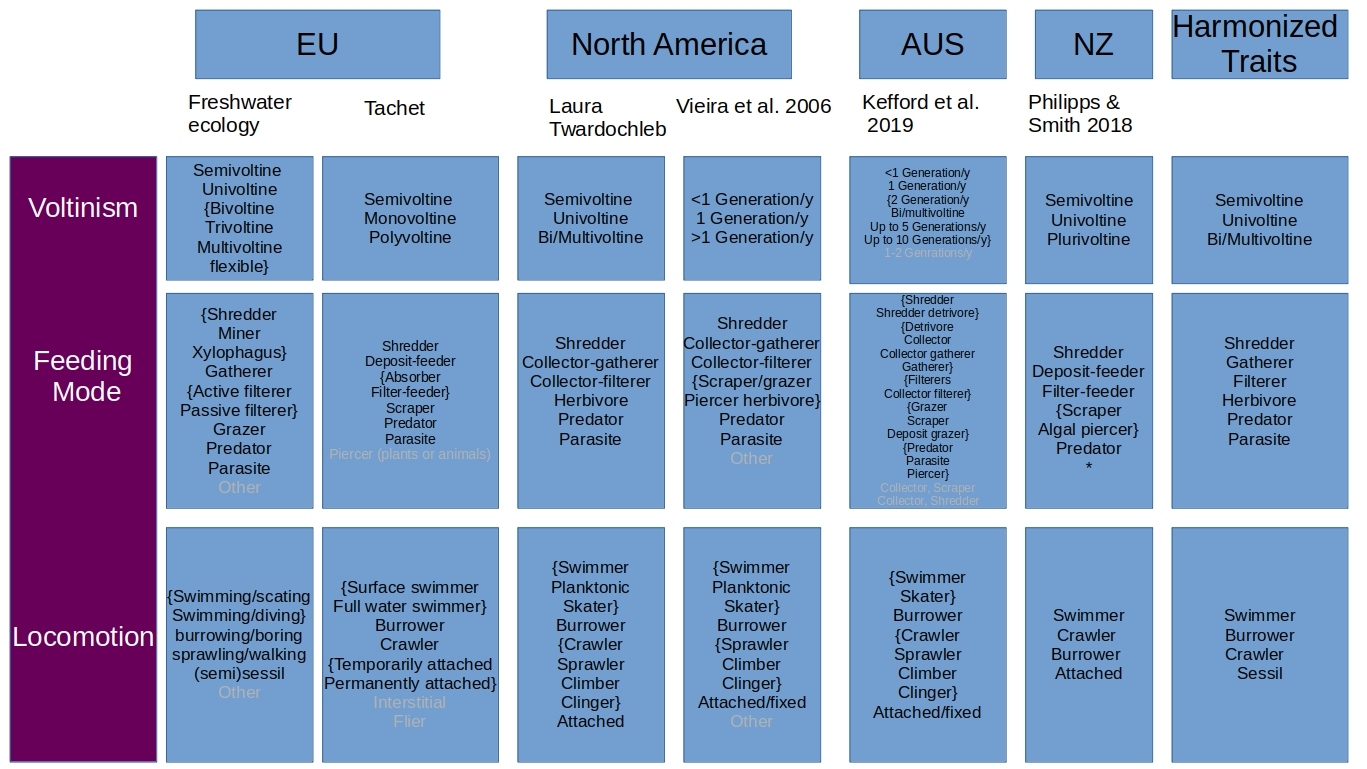
\includegraphics[width=16.5cm, height=10cm]{trait_overview1.jpg}
   \caption{Proposed harmonization scheme for the grouping features
   voltinism, feeding mode and locomotion. Shown are all traits for the 
   used grouping features in the investigated trait databases and 
   the harmonized traits in the end. Traits in curly brackets were 
   harmonized to one trait. Traits highlighted in Grey were omitted. \newline
   \textit{* Trait parasite was not available in New Zealand trait database.}
   }
   \label{fig:harmon_overview_1}
\end{figure}

\begin{figure}[H]
    \centering
    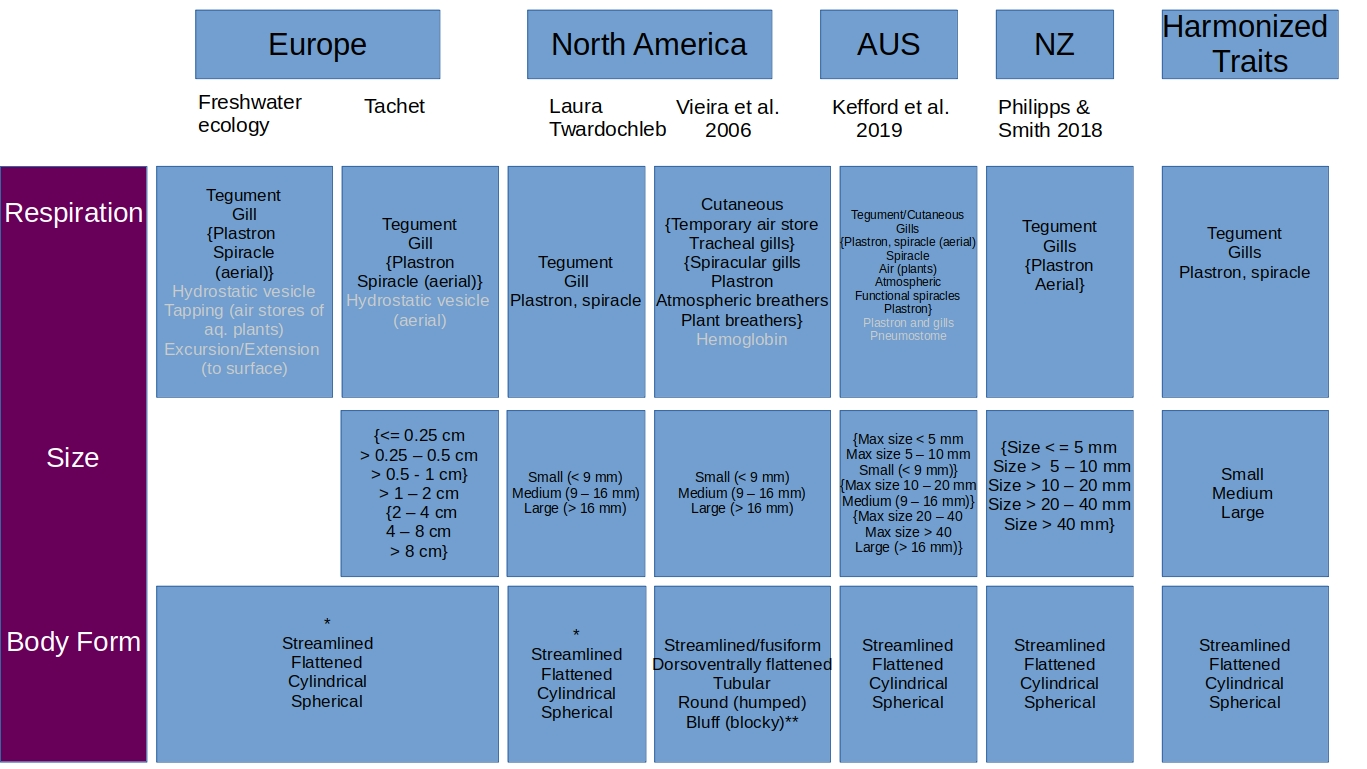
\includegraphics[width=16.5cm, height=10cm]{trait_overview2.jpg}
    \caption{Proposed harmonization scheme for the grouping features
    respiration, size and body form.\newline
    \textit{* Body form information provided by Philippe 
    Usseglio-Polatera.}\newline
    \textit{** Bluff(blocky) taxa have been reclassified
    by Philippe Usseglio-Polatera using the traits streamlined,
    flattened, cylindrical and spherical.} }
    \label{fig:harmon_overview_2}
 \end{figure}

 % !Present definition comparison 
Not only the categorization of grouping features into traits but also the definitions of individual traits varies between databases, complicating harmonization. 
%Thus, we present a differences in definitions of traits between the used databases.


\subsection{Aggregation of traits}
% TODO Describing \& testing different approaches
% TODO Problem of coding of traits

%! Description trait aggregation
% ? Aggregation considering different levels of taxonomical resolution
Traits in the processed and harmonized trait databases were aggregated to family-level using three approaches. I) taxa on species-level and genus-level were stepwise aggregated to the family-level by initially allocating them at the genus-level using the median. Then all traits were aggregated to family-level by using the mode. In cases where it was not possible to take the mode, e.g. only distinct values, multiple duplicates, or multiple duplicates and distinct values occurred the mean was taken. Hereafter, we abbreviate this aggregation type as \textit{stepwise\_agg}.
II) we directly aggregated taxa to family level using the median. We denote this aggregation as \textit{direct\_agg}. III) taxa were aggregated using a weighted approach, denoted as \textit{weighted\_agg}. The weights were determined as the ratio of how many taxa on species or genus-level were initially present per genera compared to how many taxa on species or genus-level were present after selecting only taxa with complete trait profiles. After determining the weights, taxa on species and genus-level were were aggregated to genus-level by multiplying their trait values by their respective weights. Then the weighted trait values were summed up per family for each trait.

The resulting aggregated trait values were compared to trait values assigned at family-level by experts. Trait assignments on family-level existed for the Australian database and the North American database, but only for a limited subset of grouping features and taxa. For the Australian database we could compare aggregated trait values with assigned trait values resolved at family-level for the grouping features feeding mode and size by using data from Chessman et al. % TODO Cite Chessman
% TODO: Comment here that the Chessman traits are also part of the AUS DB -> isn't this a bit a problem? Have been used in calculating
% aggregated trait values
For the North American database we could compare aggregated trait values with assigned trait values 
on family-level for the grouping features feeding mode, respiration, size, voltinism and locomotion. 
The trait information was obtained from the trait database by Pyne et al, which contains trait information
for aquatic insects resolved on genus and family-level. Trait information on family-level was available for 
94 families of which 61 (approximately 65 \%) were present in the aggregated North American trait database. 
Trait information in the Pyne database was on the nominal scale and was converted to binary traits prior to the comparison with aggregated traits values. 
% TODO: Cite Pyne 

\section{Results}
%%%%%%%%%%%%%%%%%%%%%%%%%%%%% MAIN RESULTS %%%%%%%%%%%%%%%%%%%%%%%%%%%%%
% Data preparation complex -> many decisions
% Databases are not ideal (not standardized, different trait definitions)
% Report missing information -> How many families not "get lost"
% Effect of trait aggregation
% Trait values only slightly vary between complex and direct aggregation
 % -> compare with family assignments: Roughly 25 % are classified differently
    % -> Which and why? 
    % -> Add statistical technique -> Maybe clustering?  
 % -> test with weights?
 % -> (effect of transforming binary to fuzzy codes -> US data subset test)
%%%%%%%%%%%%%%%%%%%%%%%%%%%%% MAIN RESULTS %%%%%%%%%%%%%%%%%%%%%%%%%%%%%
%!General overview, how many taxa, distinct orders, ...
\subsection{Taxonomical coverage}
Regarding the taxonomical coverage the New Zealand database has, as expected, the smallest 
taxon pool. In total 492 taxa are covered by this database. Thereof, 404 taxa resolved on species-level, 47 taxa 
on genus-level and 27 taxa on family-level. The remaining entries are on a lower taxonomical resolution. 
73 \% of taxa in the New Zealand database belong to the group of aquatic insects.
The largest taxon pool is spanned by the European trait database, with 4224 taxa of 76 different orders. 
48 \% of the taxa in this database belong to the group of aquatic insects. The European database is 
mostly on the highest taxonomical resolution possible, with 3953 taxa on species-level (approximately 93,6 \%).
253 entries are resolved on genus-level and 18 entries on family-level.
The Australian database has 1404 taxa of 64 orders. 52 \% of the taxa covered are aquatic insects. 
564 taxa are resolved on species-level, 578 on genus-level and 260 on family-level.
The North American trait database contained trait information for 3542 taxa of 42 different orders, 
although 63 \% of the taxa in the database belong to the aquatic insects. 2142 entries are on 
species-level, 1074 on genus-level and 50 on family-level. 

%! How big is the data gap?
\subsection{Completeness of trait information}
The percentage of entries with available information for the individual grouping features in the Australian, European and
North American trait databases varied between 5 \% and 99 \%. By contrast, the New Zealand trait database
contained complete trait information for 99 \% to 100 \% of their entries for the individual grouping features (\ref{tab:trait_coverage}).
The greatest data gap was for the grouping feature body form where information was only present for 7 \% of entries
in the Australian and European database, and 26 \% of entries in the North American database. % TODO: Comment in Draft file for Ralf
Selecting only taxa resolved at least at 
family-level and with complete trait profiles for the six grouping features lead to the omission of many taxa in all databases except for the New Zealand database. 
Out of the 21 orders that the New Zealand database covers, taxa of 20 orders remained after the selection process.
For most orders, all families initially included were also included after selecting taxa with complete trait profiles (table \ref{tab:fam_preproc/fam_init}).
By contrast, in the Australian database, only taxa from five orders (Ephemeroptera, Megaloptera, Odonata, Plecoptera, 
and Trichoptera) remained. Within these five orders, there was none where all families included in the database contained complete trait profiles. % Clearly the lack of data for body form results in the omission of many taxa
In the North American database, taxa of 18 orders had complete trait profiles, in the European database 9 orders. 

\begin{table}[H]
  \centering
  \caption{Percentage of entries that have information for the 
  individual grouping features per database.} 
  \label{tab:trait_coverage}
  \begin{tabular}{llr}
    \hline
  Database & Grouping feature & Trait covered [\%] \\ 
    \hline
  Australia & Body form & 5.00 \\ 
    Australia & Feeding mode & 99.00 \\ 
    Australia & Locomotion & 42.00 \\ 
    Australia & Respiration & 70.00 \\ 
    Australia & Size & 78.00 \\ 
    Australia & Voltinism & 49.00 \\ 
    Europe & Body form & 7.00 \\ 
    Europe & Feeding mode & 65.00 \\ 
    Europe & Locomotion & 33.00 \\ 
    Europe & Respiration & 56.00 \\ 
    Europe & Size & 11.00 \\ 
    Europe & Voltinism & 24.00 \\ 
    New Zealand & Body form & 100.00 \\ 
    New Zealand & Feeding mode & 99.00 \\ 
    New Zealand & Locomotion & 99.00 \\ 
    New Zealand & Respiration & 100.00 \\ 
    New Zealand & Size & 100.00 \\ 
    New Zealand & Voltinism & 100.00 \\ 
    North America & Body form & 26.00 \\ 
    North America & Feeding mode & 61.00 \\ 
    North America & Locomotion & 51.00 \\ 
    North America & Respiration & 44.00 \\ 
    North America & Size & 75.00 \\ 
    North America & Voltinism & 47.00 \\ 
    \hline
  \end{tabular}
  \end{table}

% ?Overview how complete each trait is, by order

% TODO: Mention orders that are not represented at all 
% TODO: Which entries have 0 %, which were not present initially?
\begin{table}[H]
  \centering
  \caption{Proportion of families per order that remain
  after only taxa with complete trait profiles have been selected from the total
  number of distinctive families in the databases.} 
  \label{tab:fam_preproc/fam_init}
  \begin{tabular}{lrrrr}
    \hline
  Order & Australia & New Zealand & Europe & North America \\ 
    \hline
  Amphipoda &  & 100.00 & 37.50 & 10.00 \\ 
    Anthoathecata &  & 100.00 &  &  \\ 
    Architaenioglossa &  &  &  & 100.00 \\ 
    Arhynchobdellida &  &  &  & 100.00 \\ 
    Branchiopoda &  &  &  & 100.00 \\ 
    Coleoptera &  & 88.89 & 83.33 & 15.62 \\ 
    Cycloneritida &  &  &  & 100.00 \\ 
    Decapoda &  & 100.00 &  &  \\ 
    Diptera &  & 100.00 & 46.15 & 21.62 \\ 
    Ephemeroptera & 50.00 & 100.00 & 66.67 & 73.91 \\ 
    Hemiptera &  & 50.00 & 63.64 & 47.06 \\ 
    Hexapoda &  & 100.00 &  &  \\ 
    Lepidoptera &  & 100.00 &  &  \\ 
    Littorinimorpha &  &  &  & 66.67 \\ 
    Mecoptera &  & 100.00 &  &  \\ 
    Megaloptera & 50.00 & 100.00 &  & 50.00 \\ 
    Mollusca &  & 100.00 &  &  \\ 
    Mysida &  & 100.00 &  &  \\ 
    Nemertea &  & 100.00 &  &  \\ 
    Neuroptera &  & 100.00 &  &  \\ 
    Odonata & 6.90 & 100.00 & 100.00 & 50.00 \\ 
    Oligochaeta &  & 100.00 &  &  \\ 
    Onychura &  &  &  & 100.00 \\ 
    Plecoptera & 25.00 & 100.00 & 100.00 & 88.89 \\ 
    Rhynchobdellida &  & 100.00 &  & 50.00 \\ 
    Spinicaudata &  &  &  & 100.00 \\ 
    Tanaidacea &  & 100.00 &  &  \\ 
    Trichoptera & 52.17 & 100.00 & 95.45 & 71.43 \\ 
    Venerida &  &  & 100.00 & 33.33 \\ 
     \hline
  \end{tabular}
  \end{table}

\subsection{Taxonomical overlap between trait databases}
% TODO: taxonomic overlap between databases rather small

\subsection{Deviance in trait values}
% !How many taxa end up with different trait values after aggregation?(%) 
% TODO: Improve R script
% TODO: Write paragraph
% TODO: Add graphs?
% Generally both methods result in similar values on family-level.
% When deviations, then rather small
% Complex agg: Seems to make only sense with cases where many observations 
% -> many species per Genera, many genera per family

% Deviating cases: mostly Trichoptera, North America Ephemeroptera
% No family that shows deviating results across all databases

% TODO: Comment -> Suggest to Ralf other approaches, if time test them
The \textit{stepwise\_agg} and \textit{direct\_agg} approaches yielded for the majority of taxa 
the same trait values (table \ref{tab:diff_trait_agg_methods}) across all grouping features.
The amount of cases for were the two aggregation methods resulted in different trait values varied between approximately 1 \% and 3.5 \%.
One case here is a taxa resolved on family-level with a specific trait.

% ! Which traits/grouping features show mainly different values between both aggregation methods?
% In cases were \textit{stepwise\_agg} and \textit{direct\_agg} resulted in different trait values, they mostly deviated for the grouping features feeding mode and body size. 
% Feeding mode herbivore, size medium and small were 3 families for the Australian trait database. Size medium was differently for 6 families in the European trait database. 
% Feeding mode shredder 4 times New Zealand
% Feeding mode gatherer, size small, size medium, resp gil 6 times North American
%! Taxa that were differently classified in all databases
% give Leptophelibidae example & 
% Among the differently classified taxa are mostly aquatic insects. 

There was no family that had diverging trait values produced by the aggregation methods in all databases, although for Leptophlebiidae (order Ephemeroptera) the aggregation methods produced different trait values in the European, North American and Australian trait databases.
%! How much are trait values deviating?
% TODO: Maybe leave out and put in later
% If aggregated trait values were deviating between the \textit{stepwise\_agg} and \textit{direct\_agg} they
% mostly ranged 

\begin{table}[ht]
      \centering
      \caption{Percentage of cases where the \textit{stepwise\_agg} and \textit{direct\_agg} methods 
      resulted in different trait values on family-level.}
      \label{tab:diff_trait_agg_methods}
      \begin{tabular}{lrr}
        \hline
      Database & Deviating cases [\%] & Number of cases \\ 
        \hline
      Australia & 3.52 & 483 \\ 
        Europe & 2.17 & 2024 \\ 
        New Zealand & 1.03 & 2134 \\ 
        North America & 2.66 & 2139 \\ 
        \hline
\end{tabular}
\end{table}

% ! Comparison with traits assigned on family level
\subsection{Comparison aggregated trait values and trait values assigned at family-level}

\subsubsection{Australia}

\subsubsection{North America}
Overall, approximately 21 \% of trait values evaluated at family-level by Pyne et al. were different to the trait values obtained by \textit{direct\_agg} in the North American trait database for families both databases share. Compared to the \textit{stepwise\_agg}, 22 \% of trait values from Pyne et al. were different. Trait values for body \textit{size medium} were most often deviating between the \textit{direct\_agg} and traits assigned at family-level (45.9 \% of all families, total number of taxa on family-level: 61), followed by voltinism 
\textit{univoltine} (36 \%), and feeding mode \textit{gatherer} (32.8 \%). Since both aggregation methods mostly resulted in similar trait values, differences in trait values between \textit{stepwise\_agg} and traits assigned at family-level were similar to the differences for \textit{direct\_agg}. The most deviating trait was again body \textit{size medium} (47.5 \% of all families), followed by voltinism \textit{univoltine} (37.7 \%), and \textit{size small} (29.5 \%). Among all compared traits there were always differences in aggregated trait values and
assigned values at family-level for at least families from one order. Tables S\ref{tab:SI_perc_dir_agg_expert_NOA} and S\ref{tab:SI_perc_stepwise_agg_expert_NOA} give an overview over how many families were differently evaluated by the aggregation methods compared to Pyne's database for all investigated traits.
%! Most deviating cases per order?
Regarding deviating cases per order, families from Ephemeroptera had most often different assigned trait values compared to the trait values obtained by the \textit{direct\_agg} (24.37 \% of cases, table S\ref{tab:SI_perc_dir_agg_expert_family_NOA}). For the \textit{stepwise\_agg} families from Trichoptera (24.51 \% of cases, table S\ref{tab:SI_perc_stepwise_agg_expert_family_NOA}) were deviating from the assigned trait values. For both aggregation methods families from Odonata differed the least often to the assigned trait values (16.18 \% respectively).

%! Discuss range of trait deviations
Trait values ranged between $0$ and $1$. Hence, the maximum deviation possible is 1 (100 \%). Regarding the cases with deviations in trait values between \textit{direct\_agg} and at family-level assigned traits, 26 \% of the cases showed a deviation of 100 \%, i.e. the value obtained by \textit{direct\_agg} was 0 or 1 while the value on family-level assigned was 1 or 0 (Figures S\ref{fig:trait_dev_dir_agg_feeding} to S\ref{fig:trait_dev_stepwise_agg_volt}.). Maximum deviations occurred within all orders except for Dipterans. Most often the trait \textit{size medium} (8 times, 14 \% of all maximum deviations) deviated by 100 \%, followed by the trait \textit{univoltine} (7 times, 12.3 \% of all maximum deviations) and trait \textit{size small} (7 times).

Comparison of the cases with deviations in trait values between \textit{stepwise\_agg} and at family-level assigned traits shows a s similar picture. 25.8 \% of the cases showed a deviation of 100 \%. Maximum deviations occurred as well within all orders except for Dipterans. Most often the trait \textit{size medium} (8 times, 13.3 \% of all maximum deviations) deviated by 100 \%, followed by the trait \textit{size large} (7 times, 11.7 \% of all maximum deviations), trait \textit{size small} and trait \textit{univoltine} (both 6 times, 10 \% of all maximum deviations).


% For all cases were  
% trait values from assigned traits at family-level and trait values by \textit{direct\_agg} deviated, approximately 
% 20 \% deviated by 25 \%, i.e. the aggregated value was either 0.25 or 0.75, while the assigned value at family-level was 0 or 1
% 42 \% of cases showed a deviation of 50 \%. In these cases \textit{direct\_agg} was always resulted 0.5 and family-level was 0 or 1.
% % 8.2 % of cases 75 \% deviation 

% ? Influence on hierarchical clustering -> suggest to Ralf

\subsection{Discrepencies in trait definitions}

\subsubsection{Feeding Mode}
The determination of the feeding mode of an organism is derived from the classification into functional-feeding guilds and is based on what organisms consume, their morphology of mouthparts and their feeding behavior. % TODO: cite Moog
The freshwaterecology database, the Tachet database and the North American trait database state trait explanations describing the food sources for each trait related to the feeding mode. In the North American the method of dietary intake is also roughly described (e.g. piercers pierce prey tissues and suck fluids). The other databases give no deeper description of how exactly traits of the grouping feature feeding mode are defined.
As mentioned earlier, each databases uses different traits to describe the feeding mode (\ref{fig:harmon_overview_1}). There are also gradual differences within the definitions between the traits that occur in all databases belonging to the grouping feature feeding mode. For example, in the North American trait database shredders are defined as insects that shred on decomposing vascular plant tissue. However, freshwaterecology and tachet database include both decomposing and living plant material as food source for shredders and also additionally coarse particulate organic material (CPOM). The North American trait database summarizes taxa that scrape, shred or pierce living aquatic plants with another trait termed herbivore.

The freshwaterecology database states as reference for their classification of the grouping feature feeding mode Moog et al. (\cite{moog_comprehensive_nodate}), who in turn based their classification on Cummins (\cite{cummins_trophic_1973}), Cummins and Klug (\cite{cummins_feeding_1979}), and Merrit and Cummins.
%TODO: cite Cummins & Merrit
Also in the North American database, the classification of nutritional forms is derived from the publication of Cummins (\cite{cummins_trophic_1973}).
For the New Zealand trait databases it is not explicitly stated how they derived their classification of the feeding mode.

% Tachet cites generally: Tachet H., Bournaud M., Richoux P. & Usseglio-Polatera P. (2000) - Invertébrés d'eau douce : systématique, biologie, écologie. CNRS Editions, Paris, 588 p.

% Australia: Collection of 7 different trait databases 

%\documentclass[../Draft_harmonization_paper.tex]{subfiles}



\begin{document}

% ! Things to notice
% * Feeding Mode:
% ** Often described what is consumed, different assessments (e.g. for % predator) 
% ** Seldom reference to the mouthparts (Tachet)
% Shredder definitions actually not that different
% The Australian trait database was created out of seven sub-databases. Hence some grouping features occurred multiple times with different traits.

% TODO: Mention that NOA Vieira, AUS & NZ mostly don't give precise trait definitions
% TODO: - trait does not exist in database, mention that AUS, NZ and NOA (Vieira) do not provide detailed definitions.
% TODO: Voltinism freshwaterecology -> life cycles connected with thermal conditions -> taxa classified for different floristic regions
% TODO Use abbreviation for no precise definition given
% TODO Reproduction traits not mentioned since only the differentiation differed between databases, Similarly for Body Form
% TODO Start with mentioning that two core differences can exist: 1) definitions can be different semantically; 2) traits can be combined or more differentiated 
\subsection*{Discrepancies of invertebrate trait definitions}

Definitions of grouping features and traits varied in their level of detail. The Freshwaterecology database, and databases from Tachet and Twardochleb et al. provided more detailed descriptions of their trait information compared to the databases from Vieira et al. and New Zealand. An exception is the Australian trait database which is a collection of seven trait datasets \cite{kefford_integrated_2020}. Thus, grouping features occur multiple times with varying differentiation into traits. Depending on the dataset trait information is described with more or less detail.

The definition of grouping features varied across databases mainly concerning their differentiation into traits but also in their scope. We provide a summary of discrepancies in trait definitions in the appendix (Table S\ref{stab:trait_definitions}). Both, differences in differentiation and scope can lead to discrepancies in trait definitions. For example, for the grouping feature feeding mode discrepancies arise because traits are assigned in different ways. Tachet defines predators as carvers, engulfers and swallowers. By contrast, in the North American (Twardochleb) database predators are defined as engulfers and carnivorous piercers. In turn, in the Tachet database, piercers are defined as a separate trait encompassing herbivorous and carnivorous piercers. Furthermore, the scope in the Freshwaterecology database for feeding mode is primarily on the food source of a species (except for filterers), while the other databases focus on the strategies of food acquisition. Therefore, the Freshwaterecology database defines e.g. predator as "eating from prey", while the other databases use the mouthpart morphology as basis of their definition. The Tachet database captures the food source in an additional grouping feature. Varying levels of differentiation are also present in all other investigated grouping features between the trait databases (Table \ref{tab:trait_databases_coding_differentiation} and Table S\ref{stab:trait_definitions}). Locomotion definitions differ also in scope between databases. Freshwaterecology and New Zealand databases describe locomotion as the way of movement of an organism, Tachet as substrate relation, the North American (Vieira) as how organisms deal with flow, Australia as attachment, and the North American (Twardochleb) database includes among the way of movement also the location of movement. Similarly, regarding reproduction trait databases differ in their scope. Reproduction is captured in one grouping feature and defined as location of oviposit clutches and mode of reproduction in the Freshwaterecology and Tachet databases. North America (Vieira) provides information on the oviposition location but not on reproductive behavior. The Australian database report traits for reproductive behavior but also on oviposition site. The New Zealand database distinguishes three grouping features related to reproduction: reproductive technique, oviposition site (e.g. water surface, terrestrial), and egg/egg mass (e.g. free, cemented).

Various codings of traits are used throughout the databases (e.g. binary, fuzzy, continuous). The freshwaterecology and Australian use different codings in their databases. Tachet and the New Zealand database use exclusively fuzzy coding. Both North American trait databases contain categorical grouping features that can be converted into traits using a binary coding (Table \ref{tab:trait_databases_coding_differentiation}). Binary coding represents a simple approach in which a taxon either expresses a trait or not. Fuzzy coding characterizes the affinity of an organism to exert a certain trait. It is used to account for plasticity in traits, e.g. taking into account that traits can change over the development time of an organism. Usually, fuzzy coded affinities are converted into proportional values. Continuous coding is used for traits like body size.

% * Feeding mode:
% \begin{itemize}
%     \item freshwaterecology: describes primarily the food sources of a species, (e.g. algal tissues, CPOM, fallen leaves), except for filterers. Source: \cite{moog_comprehensive_nodate}
%     \item tachet: describes strategy/strategies adopted by the taxa for acquiring food, (e.g. taking into account mouthpart morphology). The food preference/food source has been described separately as a trait in Tachet et al. Source: \cite{usseglio-polatera_biomonitoring_2000}
%     \item North America (Twardochleb): Differentiates according to mode of food acquisition and food source, Source: \cite{cummins_trophic_1973}
%     \item North America (Vieira): Method of food collection based on mouthparts(termed feeding guild based)
%     \item Australia: Description of food source (e.g. Schäfer) also based on food acquisition (mouthpart morphology)
%     \item New Zealand: Description based on food description 
% \end{itemize}

% * Voltinism: 
% Not many differences
% \begin{itemize}
%     \item Freshwaterecology: taxa classified on floristic regions (e.g arctic, boreal). Six traits to describe voltinism. Distinguish Bivoltine, trivoltine and multivoltine in contrast to all other databases
%     \item ?Reproductive cycle vs. generations per year 
%     \item 
% \end{itemize}

% * Locomotion:
% differentiation varies between databases 
% \begin{itemize}
%     \item freshwaterecology: Way of movement of an organism
%     \item tachet: locomotion and substrate relation
%     \item North America (Twardochleb): Termed habit; way of movement and where (crawler -> floating leaves, fine sediments); Source: % Cummins & Merrit 2008
%     \item North America (Vieira): Habit -> how to deal with flow
%     \item Australia: Attachment
%     \item New Zealand: Way of movement of organism within its habitat. Trait termed attachment to substrate 
% \end{itemize}

% None of the seven grouping features compared here has the same differentiation of traits across all databases (Table \ref{tab:trait_databases})
% Table with diff trait states and coding
\begin{landscape}
    \begin{longtable}{m{2.5cm}|m{1.8cm}|m{2.3cm}|m{1.8cm}|m{3cm}|m{2cm}|m{2cm}|m{1.8cm}}
    \caption{Number of traits per grouping feature and type of coding of the traits for the respective grouping feature per database.}
    \endfirsthead
    \toprule[.1em]
    \label{tab:trait_databases_coding_differentiation}
    Database & Feeding Mode & Voltinism & Locomotion & Respiration & Reproduction & Size & Body Form \\ 
    \toprule[.1em]
    \multirow{2}{*}[-5mm]{ \specialcell{Freshwater- \\ ecology}} & 
    10 & 
    6 &
    6 & 
    7 & 
    9 & 
    - & 
    - 
    \\
    \cline{2-8} & 
    \specialcell{10 point \\ assignment \\ system} &
    \specialcell{single category \\ assignment \\ system} &
    \specialcell{10 point \\ assignment \\ system} &
    \multicolumn{2}{c |}{\specialcell{presence/absence assignment \\ system}} &
    - & 
    - \\
    \hline
    \hline
    \multirow{2}{*}{Tachet} & 
    7 & 
    3 &
    8 & 
    5 & 
    8 & 
    7 & 
    - 
    \\
    \cline{2-8} &
    \multicolumn{2}{c |}{fuzzy $[0-3]$} &
    fuzzy $[0-5]$ & 
    \multicolumn{3}{c |}{fuzzy $[0-3]$} & 
    -
    \\
    \hline
    \hline
    \multirow{2}{*}{\specialcell{North America \\ (Twardochleb)}} & 
    6 & 
    3 &
    10 & 
    3 & 
    10 & 
    3 & 
    - 
    \\
    \cline{2-8} &
    \multicolumn{6}{c |}{binary} &
    -
    \\
    \hline
    \hline
    \multirow{2}{*}{\specialcell{North America \\ (Vieira)}} & 
    8 & 
    3 &
    9 & 
    8 & 
    10 & 
    3 & 
    5 
    \\
    \cline{2-8} &
    \multicolumn{7}{c }{binary}
    \\
    \hline
    \hline
    \multirow{2}{*}[-4mm]{Australia} & 
    16 \textsuperscript{\textit{a}} & 
    7 &
    9 & 
    10 &
    13 \textsuperscript{\textit{b}} & 
    9 & 
    4
    \\
    \cline{2-8} & 
    \multicolumn{2}{c |}{\specialcell{binary; proportional $[0 - 1]$; \\ fuzzy $[0 - 3]$}} & 
    binary; fuzzy $[0 - 3]$ & 
    \specialcell{binary; proportional \\ scale $[0 - 1]$; \\ fuzzy $[0 - 3]$} & 
    categorical & 
    \specialcell{binary; \\ continuous; \\ fuzzy $[0 - 3]$} & 
    fuzzy codes $[0-3]$
    \\
    \hline
    \hline
    \multirow{2}{*}{New Zealand} & 
    6 & 
    3 & 
    4 & 
    4 & 
    4 & 
    5 & 
    4
    \\
    \cline{2-8} & 
    \multicolumn{7}{c }{fuzzy $[0-3]$}
    \\
    \bottomrule
    \end{longtable}
    \begin{minipage}{\linewidth}\small
        \textit{a} Some of the traits were similar (e.g. trait \textit{Shredder}, \textit{Shredder, Detrivore}, and \textit{Collector, Shredder}).
        \newline
        \textit{b} Many traits were rather comments than traits in the original database and were not considered.
    \end{minipage}
\end{landscape}

% ! Things to notice
% * Feeding Mode:
% ** Often described what is consumed, different assessments (e.g. for % predator) 
% ** Seldom reference to the mouthparts (Tachet)
% Shredder definitions actually not that different

% The Australian trait database was created out of seven sub-databases. Hence some grouping features occurred multiple times with different traits.

\end{document}


\newpage
\printbibliography

\section{Supporting Information}

\begin{table}[H]
  \centering
  \caption{Percentage of families differently evaluated by 
  \textit{direct\_agg} and Pyne et al. for all compared traits.} 
  \label{tab:SI_perc_dir_agg_expert_NOA}
  \begin{tabular}{lr}
    \hline
  Trait & Families differently evaluated [\%] \\ 
    \hline
    size\_medium & 45.90 \\ 
    volt\_uni & 36.07 \\ 
    feed\_gatherer & 32.79 \\ 
    size\_small & 31.15 \\ 
    size\_large & 22.95 \\ 
    locom\_crawl & 22.95 \\ 
    volt\_bi\_multi & 22.95 \\ 
    resp\_teg & 22.95 \\ 
    resp\_gil & 21.31 \\ 
    feed\_filter & 16.39 \\ 
    feed\_herbivore & 16.39 \\ 
    volt\_semi & 14.75 \\ 
    locom\_swim & 13.11 \\ 
    feed\_shredder & 13.11 \\ 
    locom\_burrow & 9.84 \\ 
    resp\_pls\_spi & 8.20 \\ 
    feed\_predator & 8.20 \\ 
     \hline
  \end{tabular}
  \end{table}

\begin{table}[H]
    \centering
    \caption{Percentage of families differently evaluated by
    \textit{stepwise\_agg} and Pyne et al.for all compared traits.} 
    \label{tab:SI_perc_stepwise_agg_expert_NOA}
    \begin{tabular}{lr}
      \hline
    Trait & Families differently evaluated [\%] \\ 
      \hline
    size\_medium & 47.54 \\ 
      volt\_uni & 37.70 \\ 
      size\_small & 29.51 \\ 
      resp\_gil & 29.51 \\ 
      resp\_teg & 29.51 \\ 
      feed\_gatherer & 29.51 \\ 
      size\_large & 26.23 \\ 
      locom\_crawl & 24.59 \\ 
      volt\_bi\_multi & 22.95 \\ 
      volt\_semi & 16.39 \\ 
      feed\_filter & 16.39 \\ 
      feed\_herbivore & 14.75 \\ 
      locom\_swim & 13.11 \\ 
      feed\_shredder & 13.11 \\ 
      locom\_burrow & 9.84 \\ 
      resp\_pls\_spi & 9.84 \\ 
      feed\_predator & 9.84 \\ 
       \hline
    \end{tabular}
\end{table}

\begin{table}[H]
  \centering
  \caption{Percentage of families differently evaluated
  by \textit{direct\_agg} and Pyne et al. for all compared orders.} 
  \label{tab:SI_perc_dir_agg_expert_family_NOA}
  \begin{tabular}{lr}
  \hline
  Order & Families differently evaluated direct\_agg [\%] \\ 
  \hline
  Ephemeroptera & 24.37 \\ 
    Coleoptera & 23.53 \\ 
    Megaloptera & 23.53 \\ 
    Trichoptera & 21.24 \\ 
    Diptera & 20.59 \\ 
    Plecoptera & 19.85 \\ 
    Hemiptera & 16.47 \\ 
    Odonata & 16.18 \\ 
  \hline
  \end{tabular}
  \end{table}

\begin{table}[H]  
  \centering
  \caption{Percentage of families differently evaluated
  by \textit{stepwise\_agg} and Pyne et al. for all compared orders.} 
  \label{tab:SI_perc_stepwise_agg_expert_family_NOA}
  \begin{tabular}{lr}
  \hline
  Order & Families differently evaluated stepwise\_agg [\%] \\ 
  \hline
  Trichoptera & 24.51 \\ 
    Ephemeroptera & 23.95 \\ 
    Coleoptera & 23.53 \\ 
    Megaloptera & 23.53 \\ 
    Hemiptera & 21.18 \\ 
    Diptera & 20.59 \\ 
    Plecoptera & 19.85 \\ 
    Odonata & 16.18 \\ 
  \hline
  \end{tabular}
  \end{table}

\begin{figure}[H]
  \centering
  \caption{Deviance of trait values obtained with \textit{direct\_agg} compared to at family level assigned traits by Pyne et al. \newline
  \textit{N} denotes the number of families per order.}
  \label{fig:trait_dev_dir_agg_feeding}
  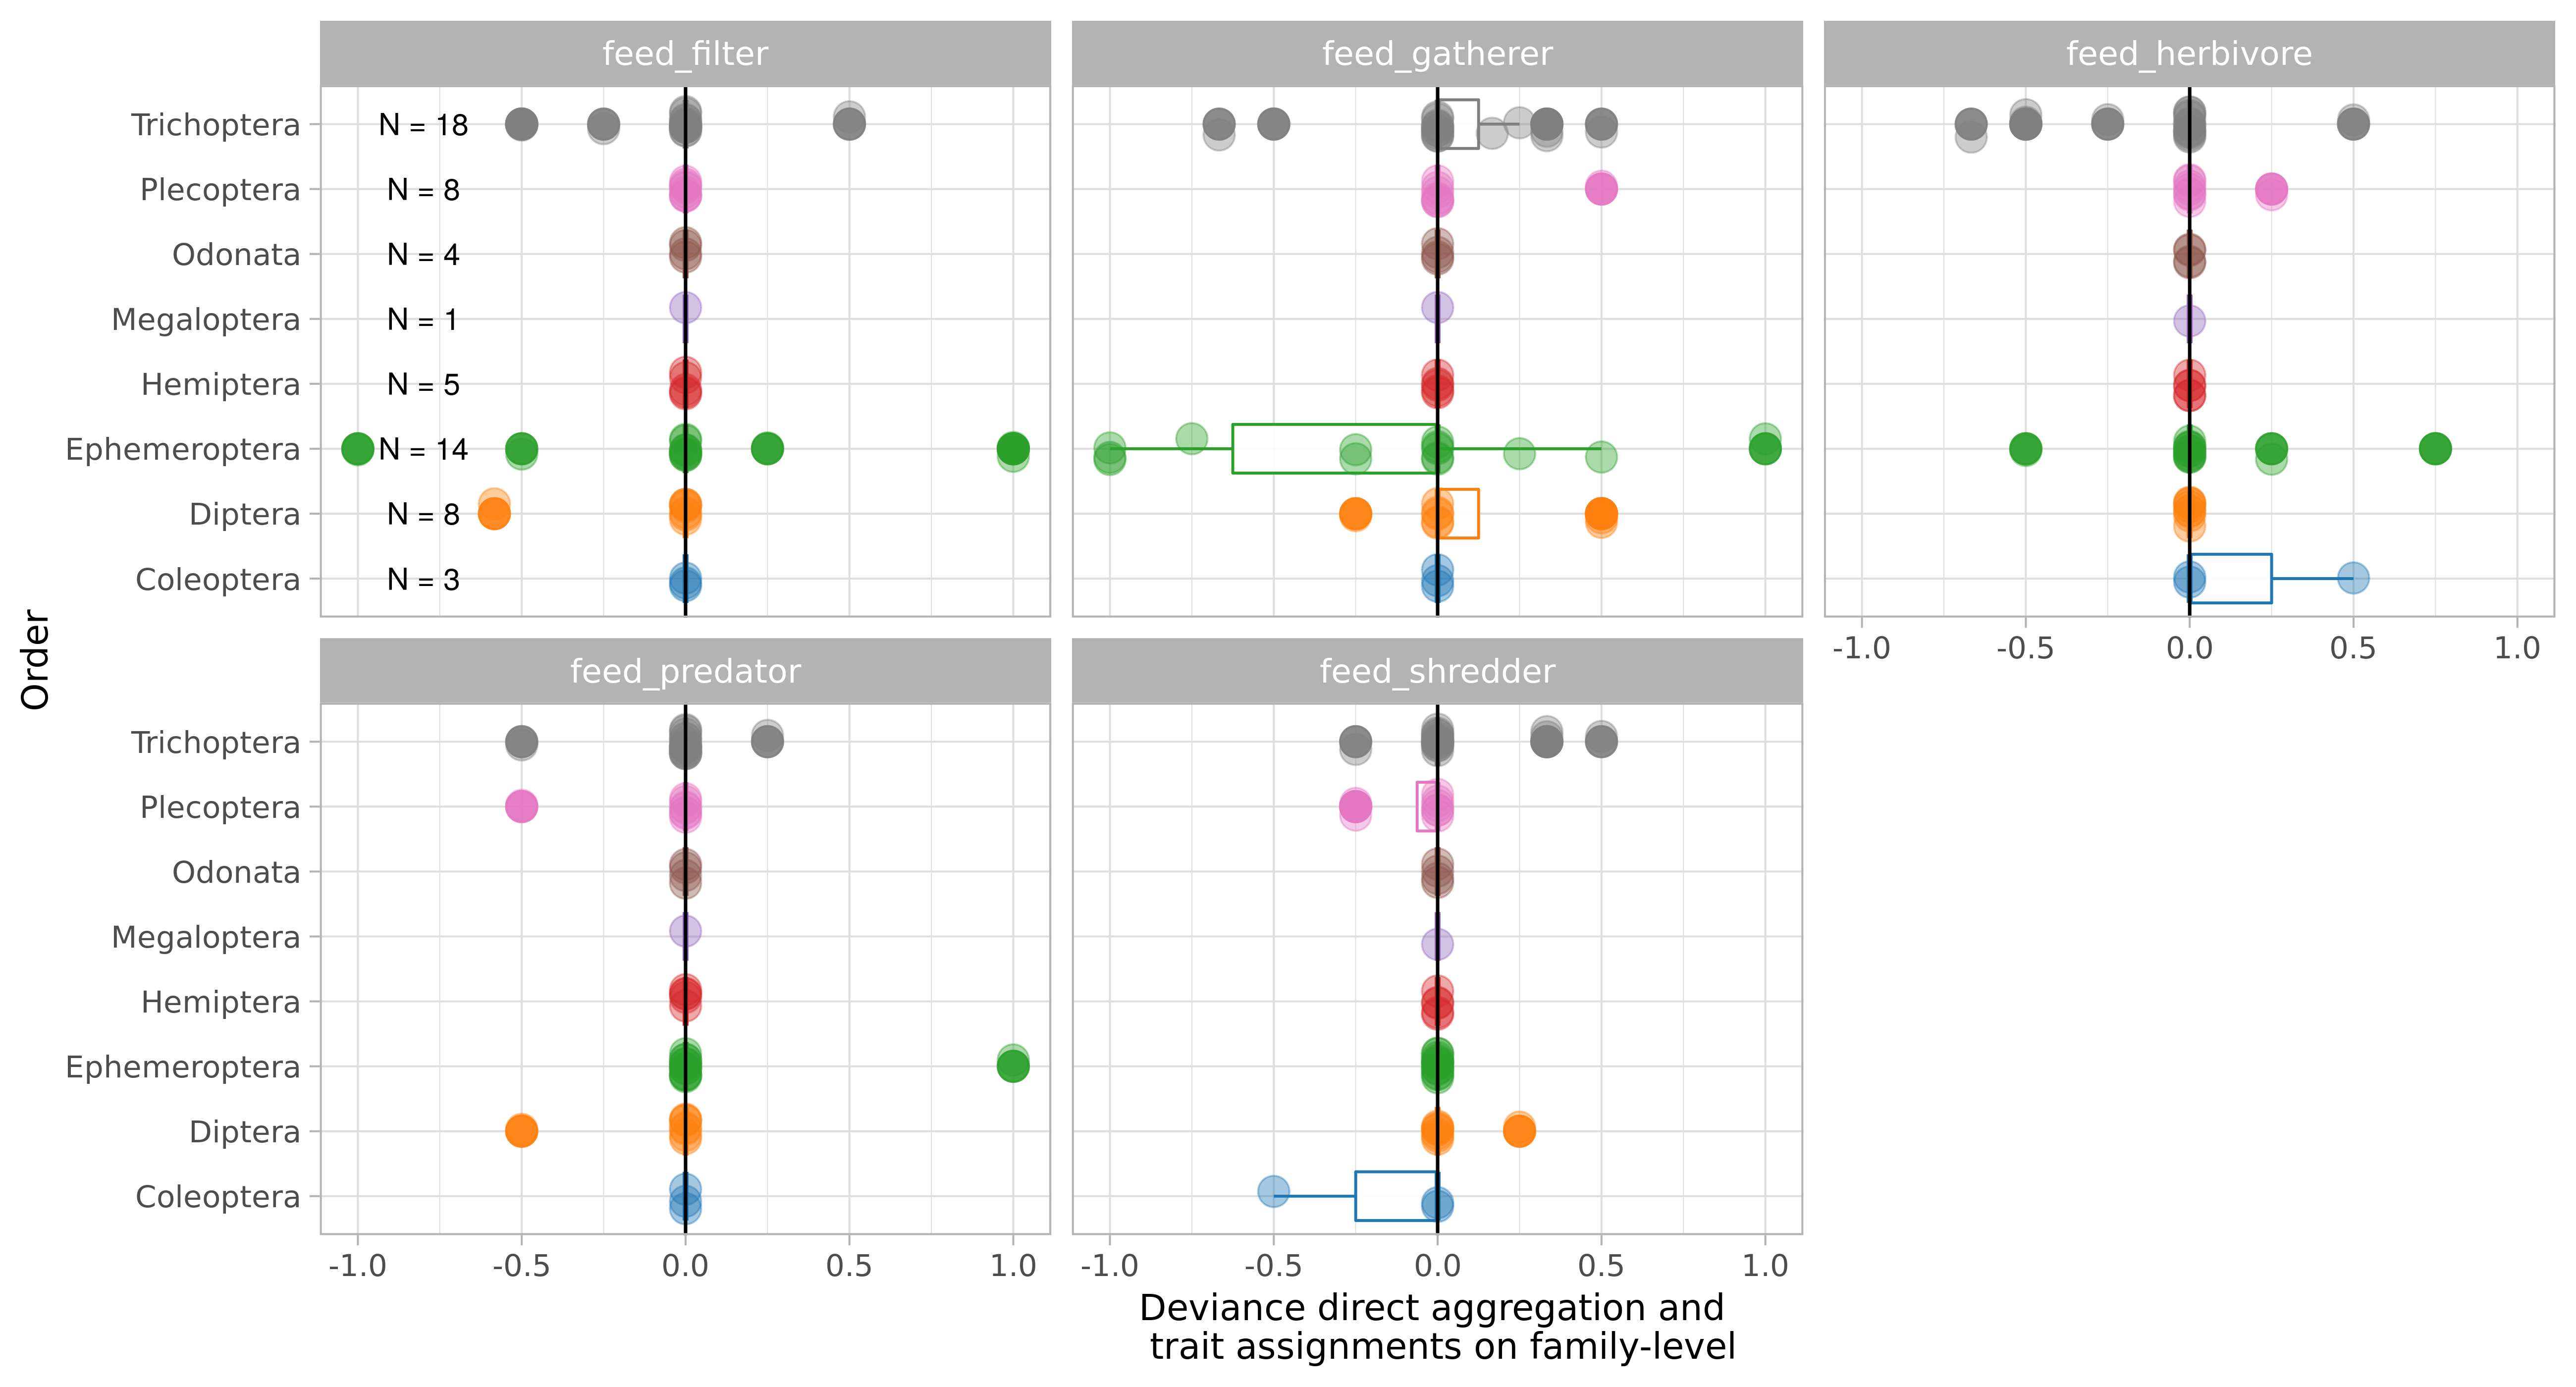
\includegraphics[width=14cm, height=7.5cm]{trait_deviations_dir_famlvl_feed.png}
\end{figure}

\begin{figure}[H]
  \centering
  \caption{.}
  \label{fig:trait_dev_dir_agg_locom}
  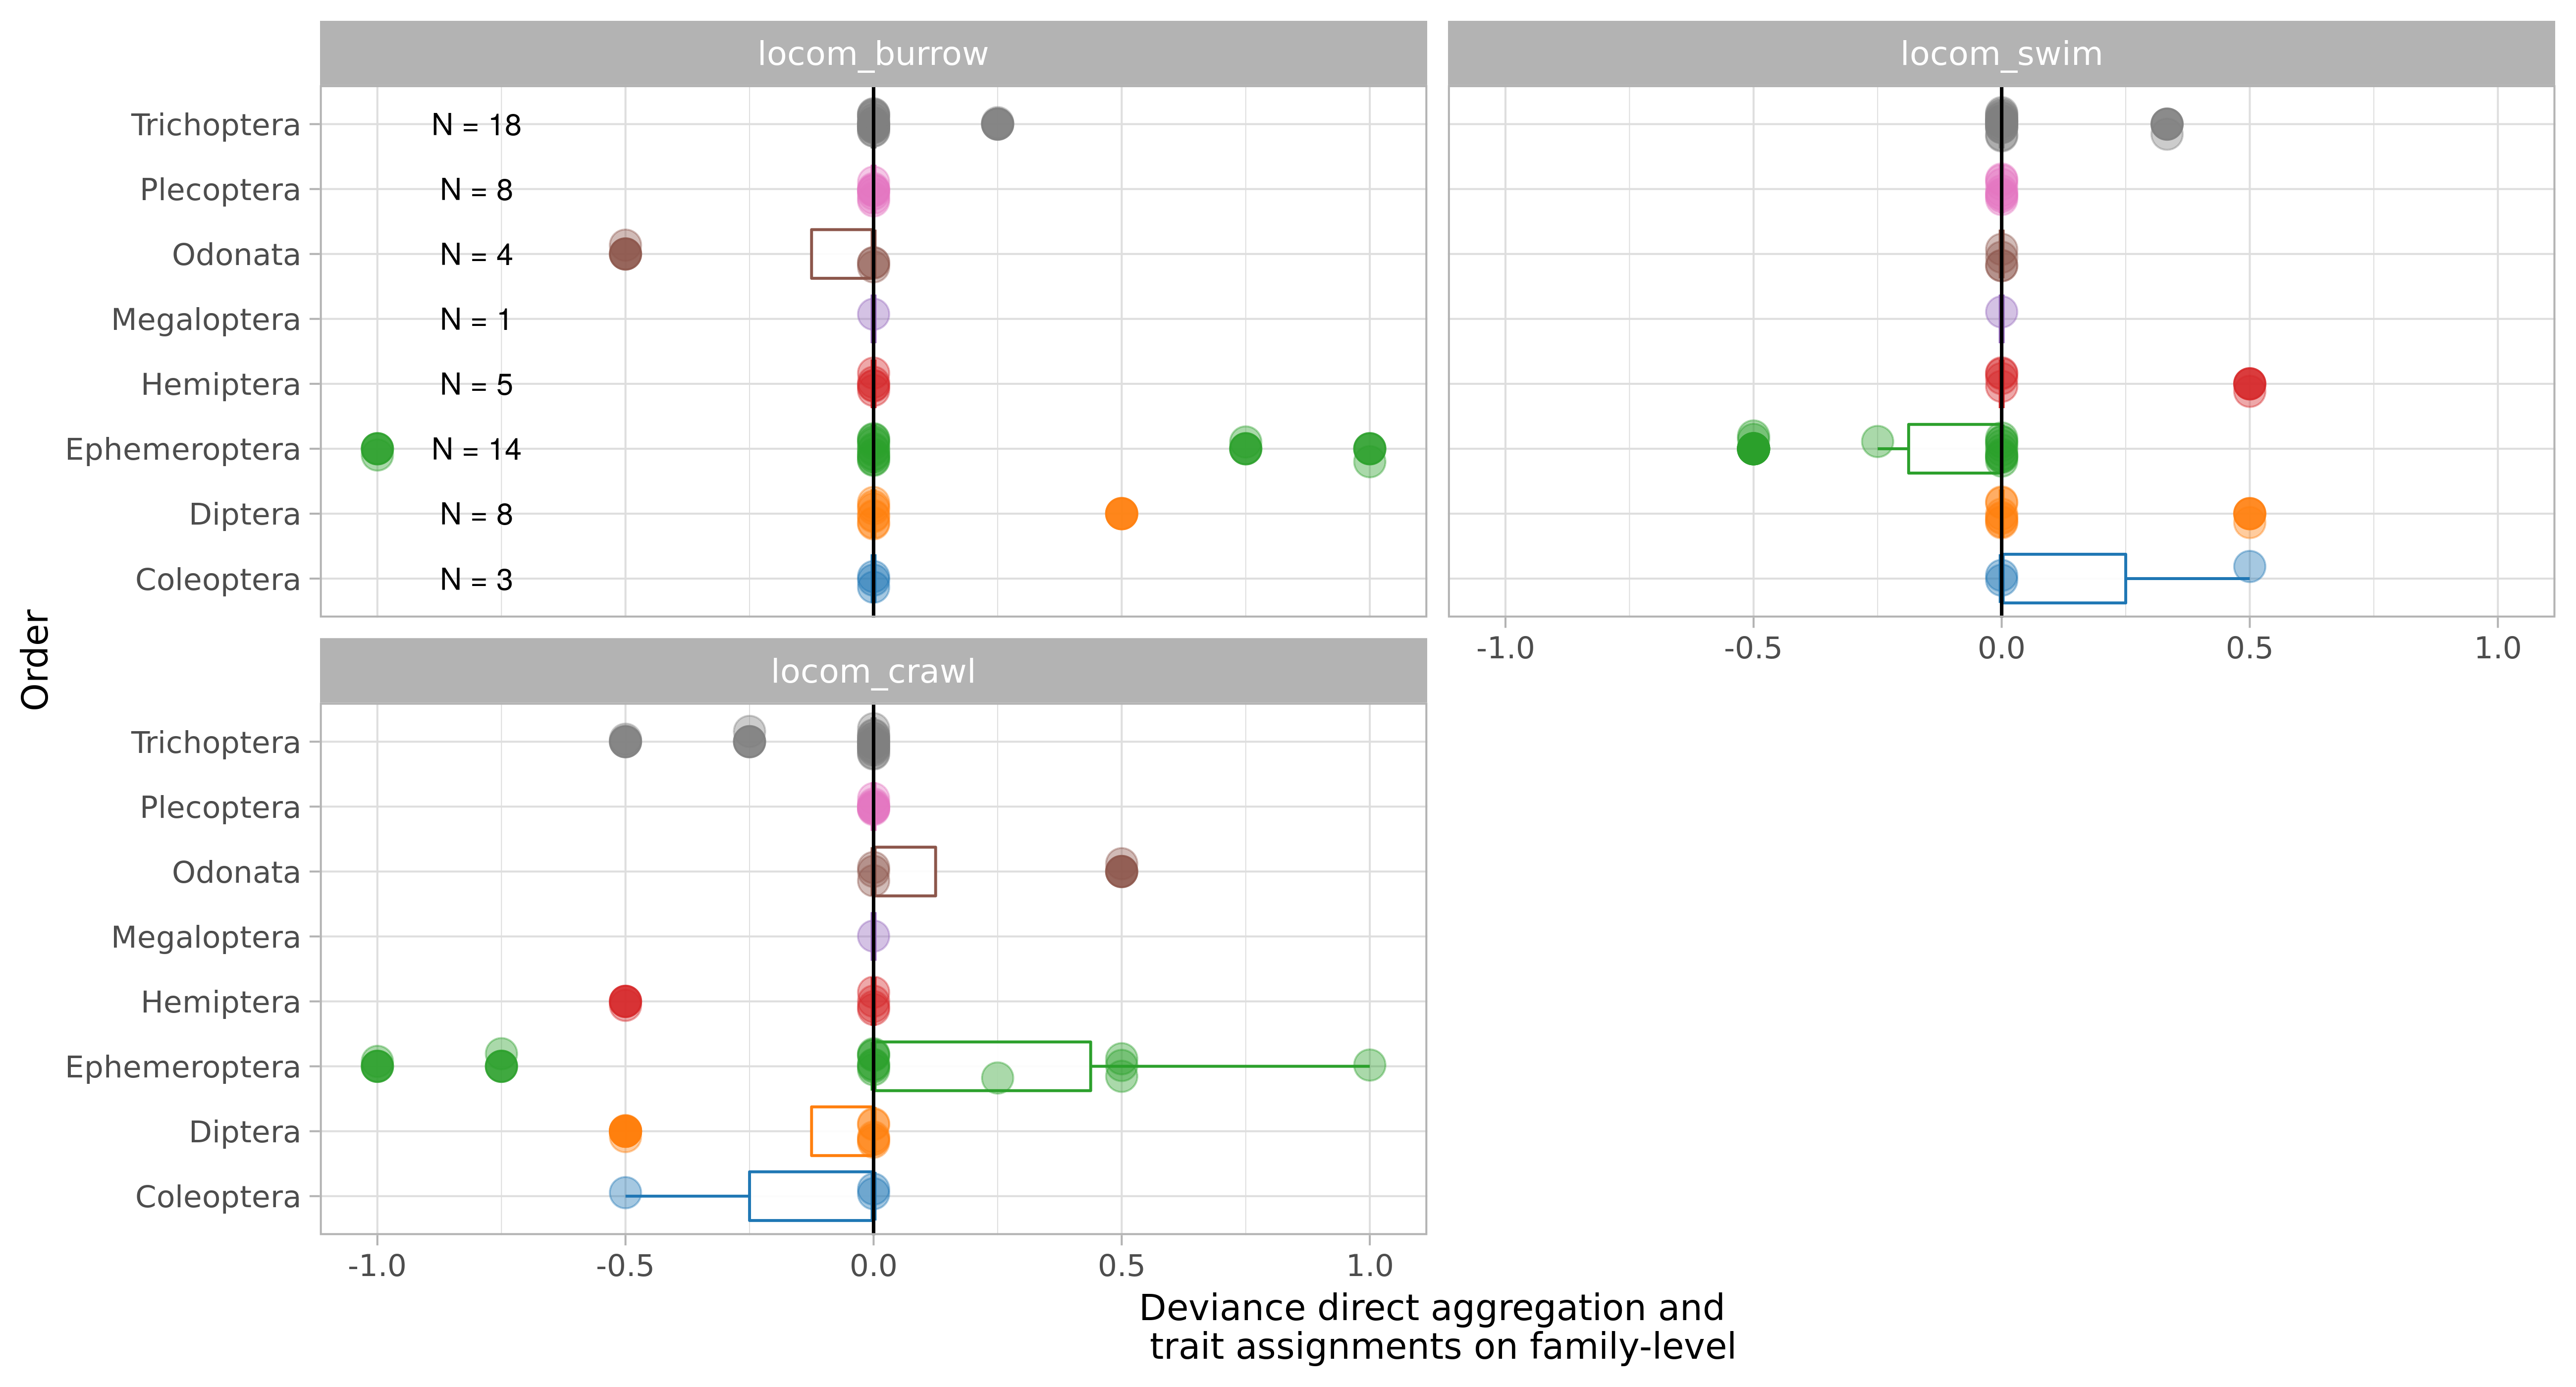
\includegraphics[width=14cm, height=7.5cm]{trait_deviations_dir_famlvl_locom.png}
\end{figure}

\begin{figure}[H]
  \centering
  \caption{.}
  \label{fig:trait_dev_dir_agg_resp}
  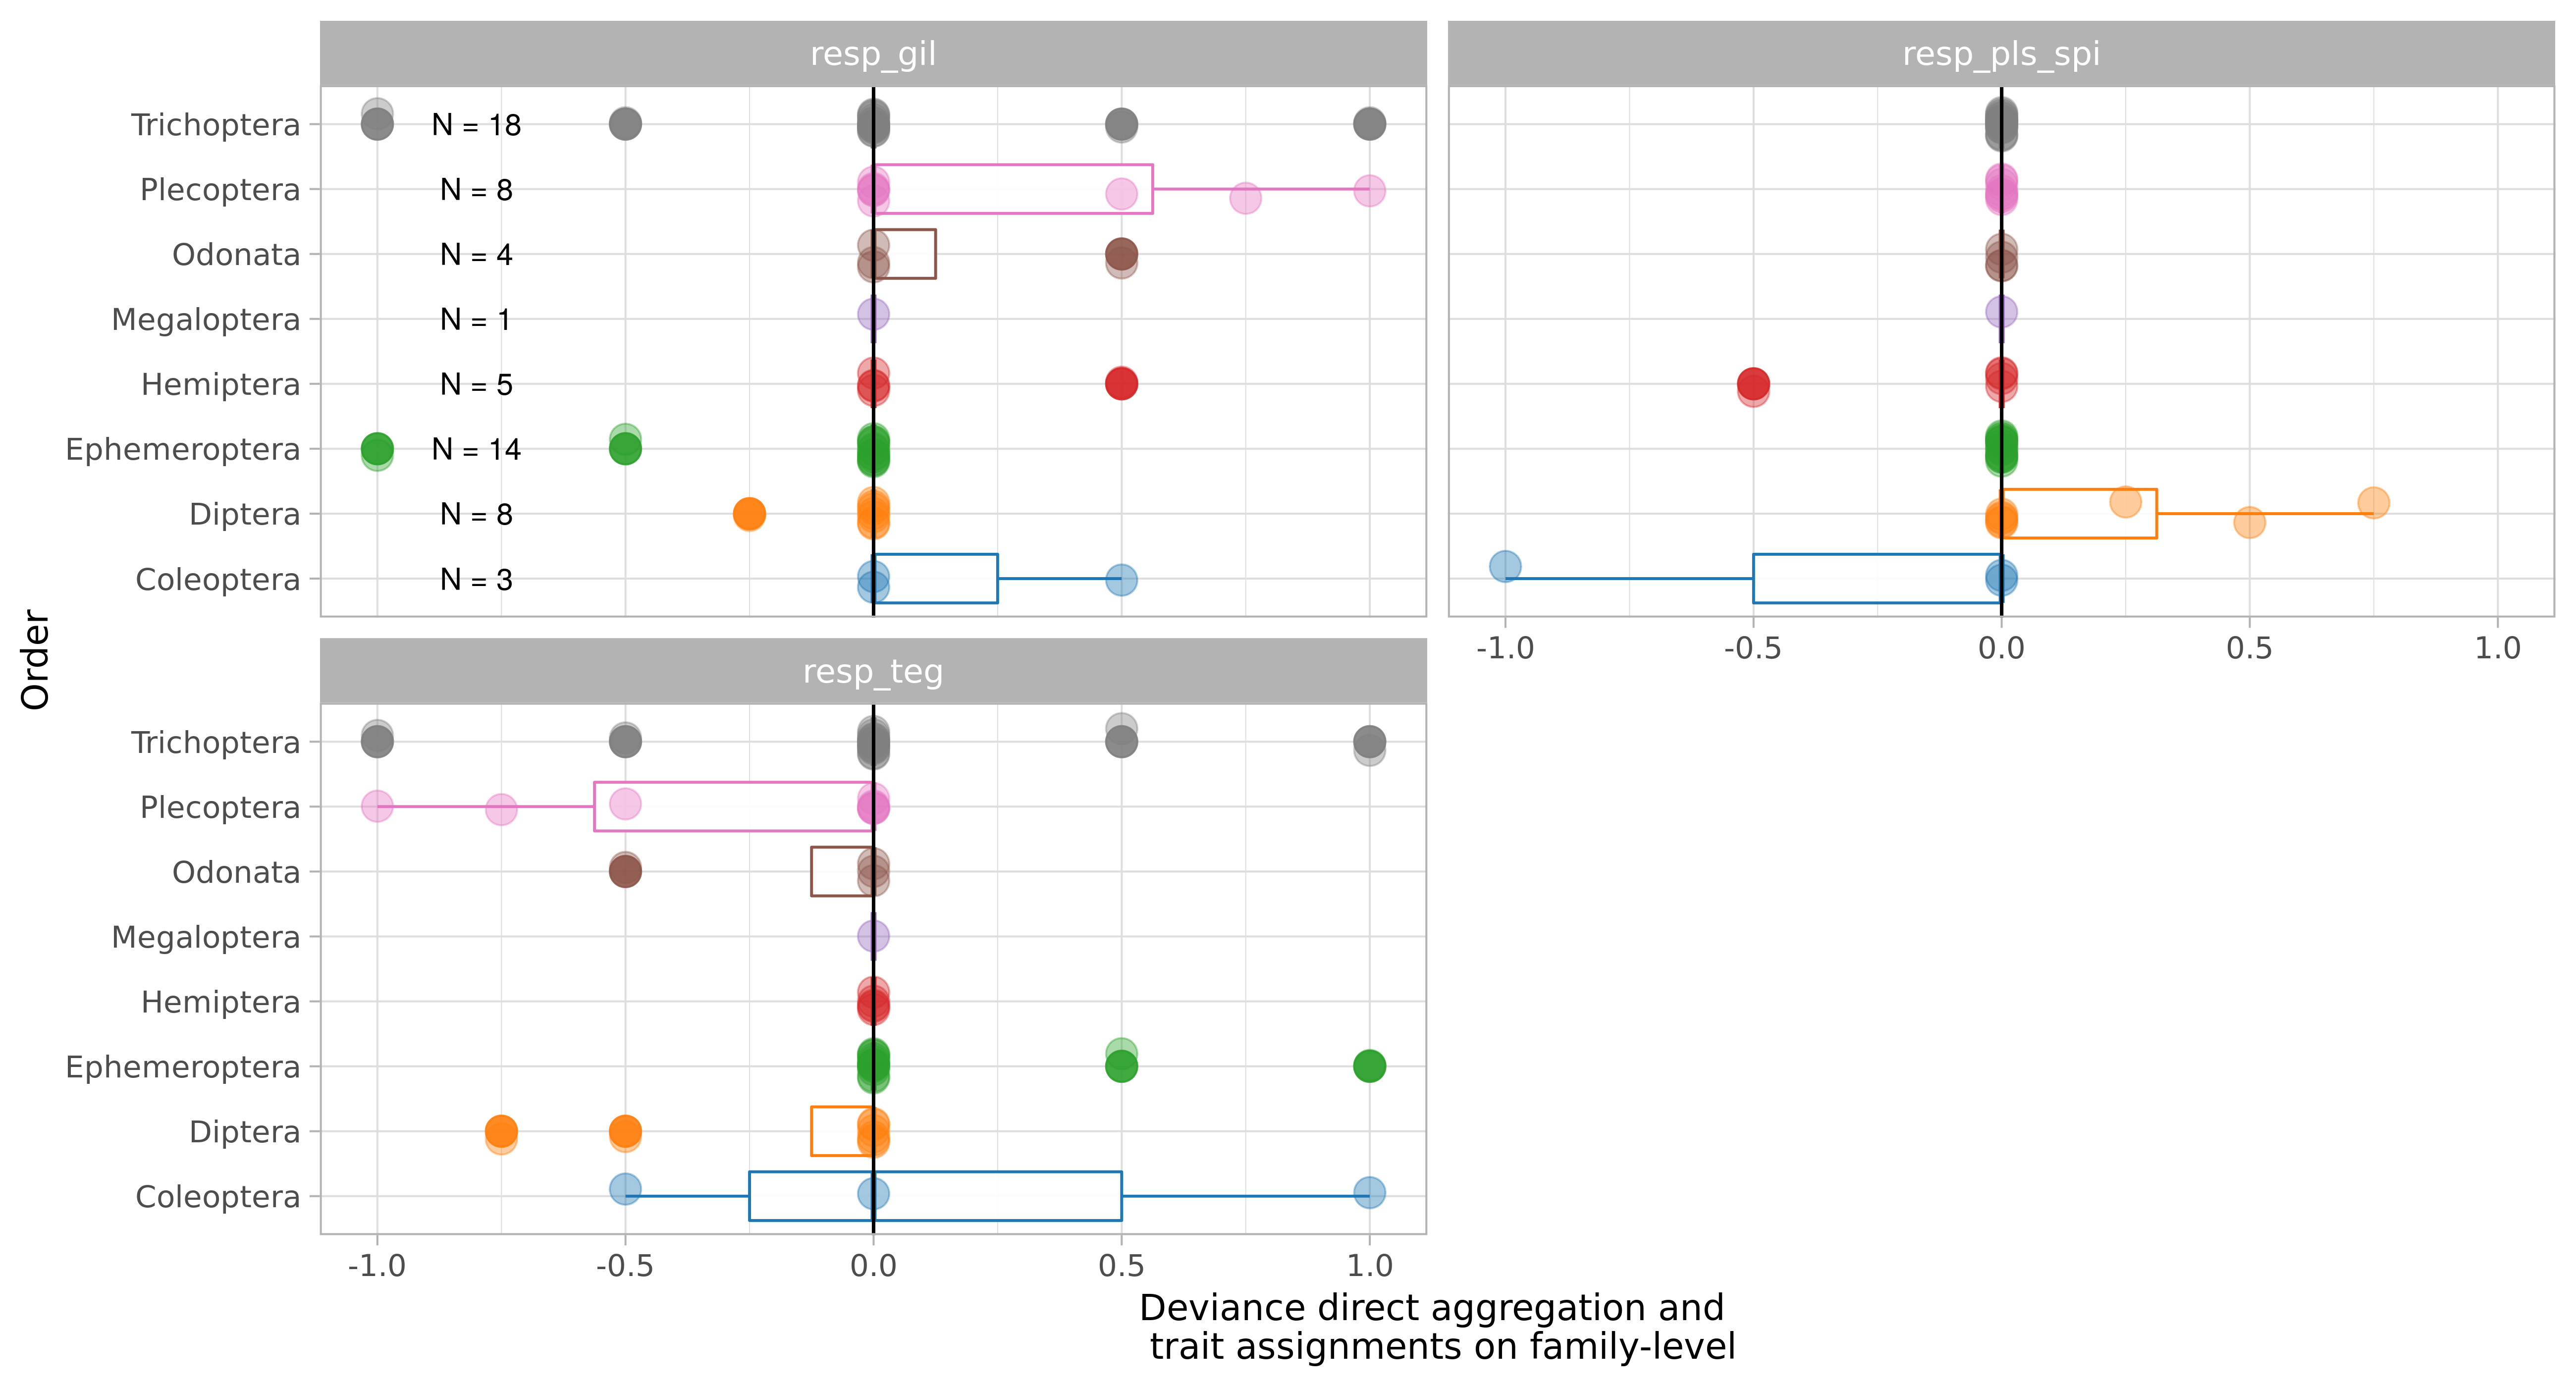
\includegraphics[width=14cm, height=7.5cm]{trait_deviations_dir_famlvl_resp.png}
\end{figure}

\begin{figure}[H]
  \centering
  \caption{.}
  \label{fig:trait_dev_dir_agg_size}
  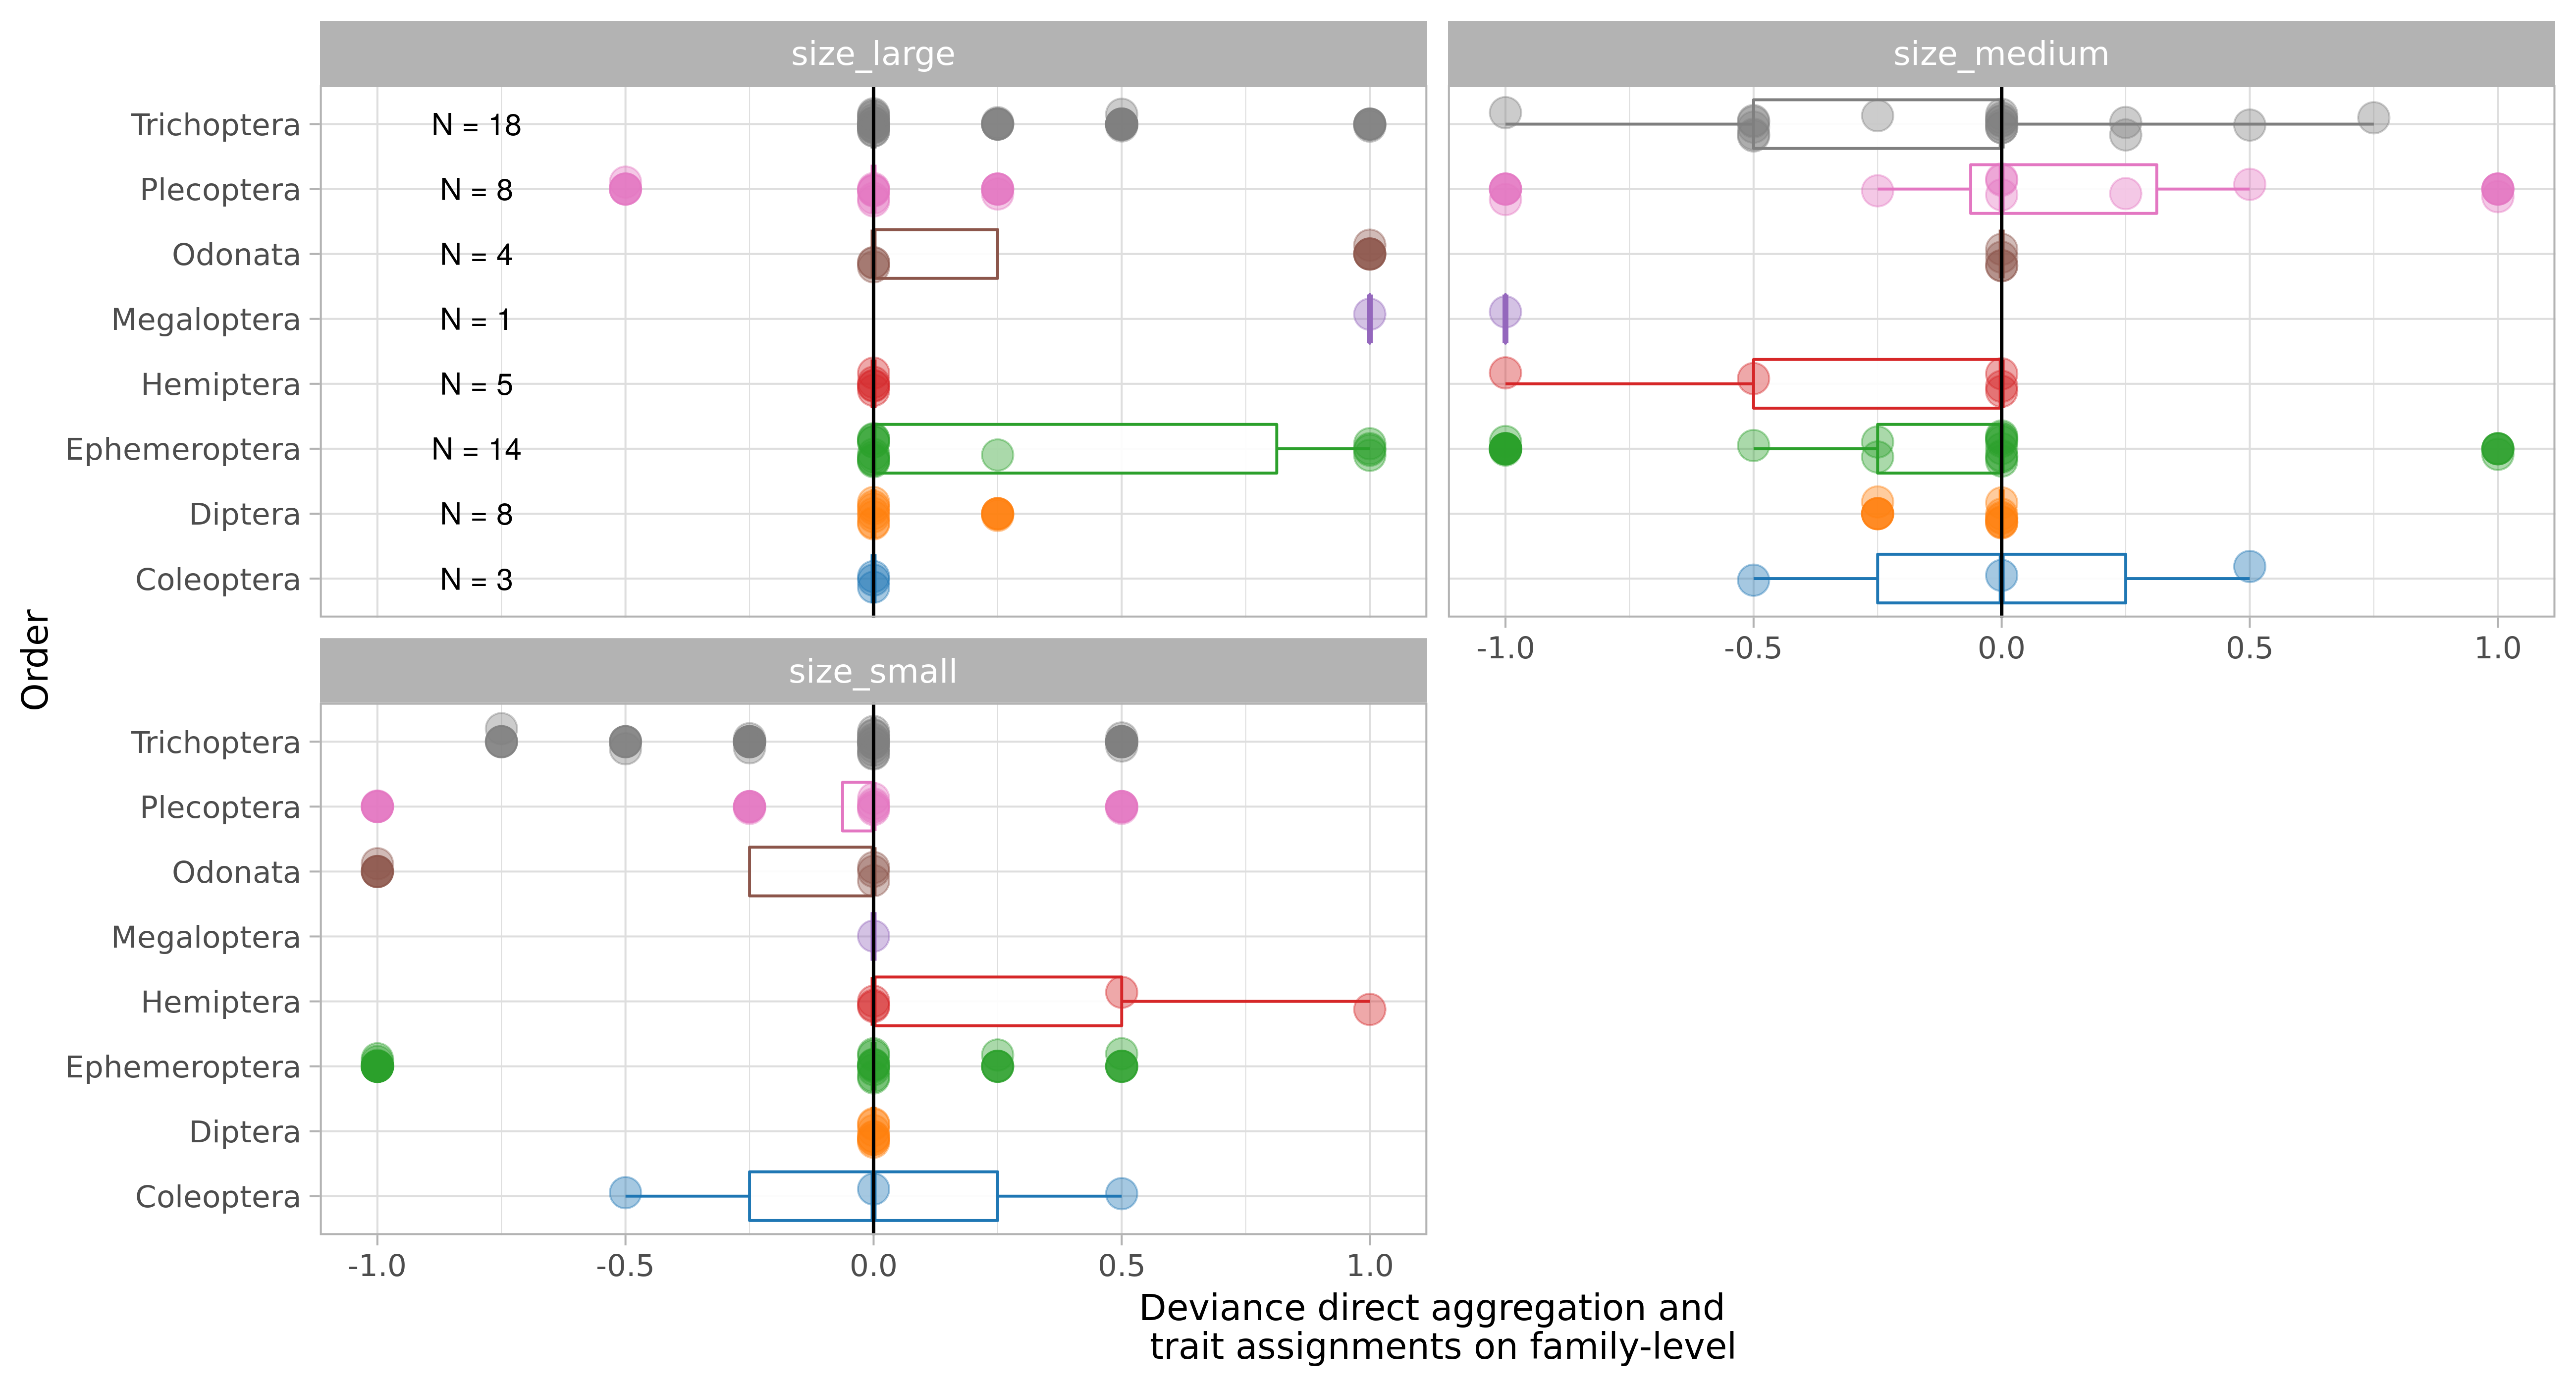
\includegraphics[width=14cm, height=7.5cm]{trait_deviations_dir_famlvl_size.png}
\end{figure}

\begin{figure}[H]
  \centering
  \caption{.}
  \label{fig:trait_dev_dir_agg_volt}
  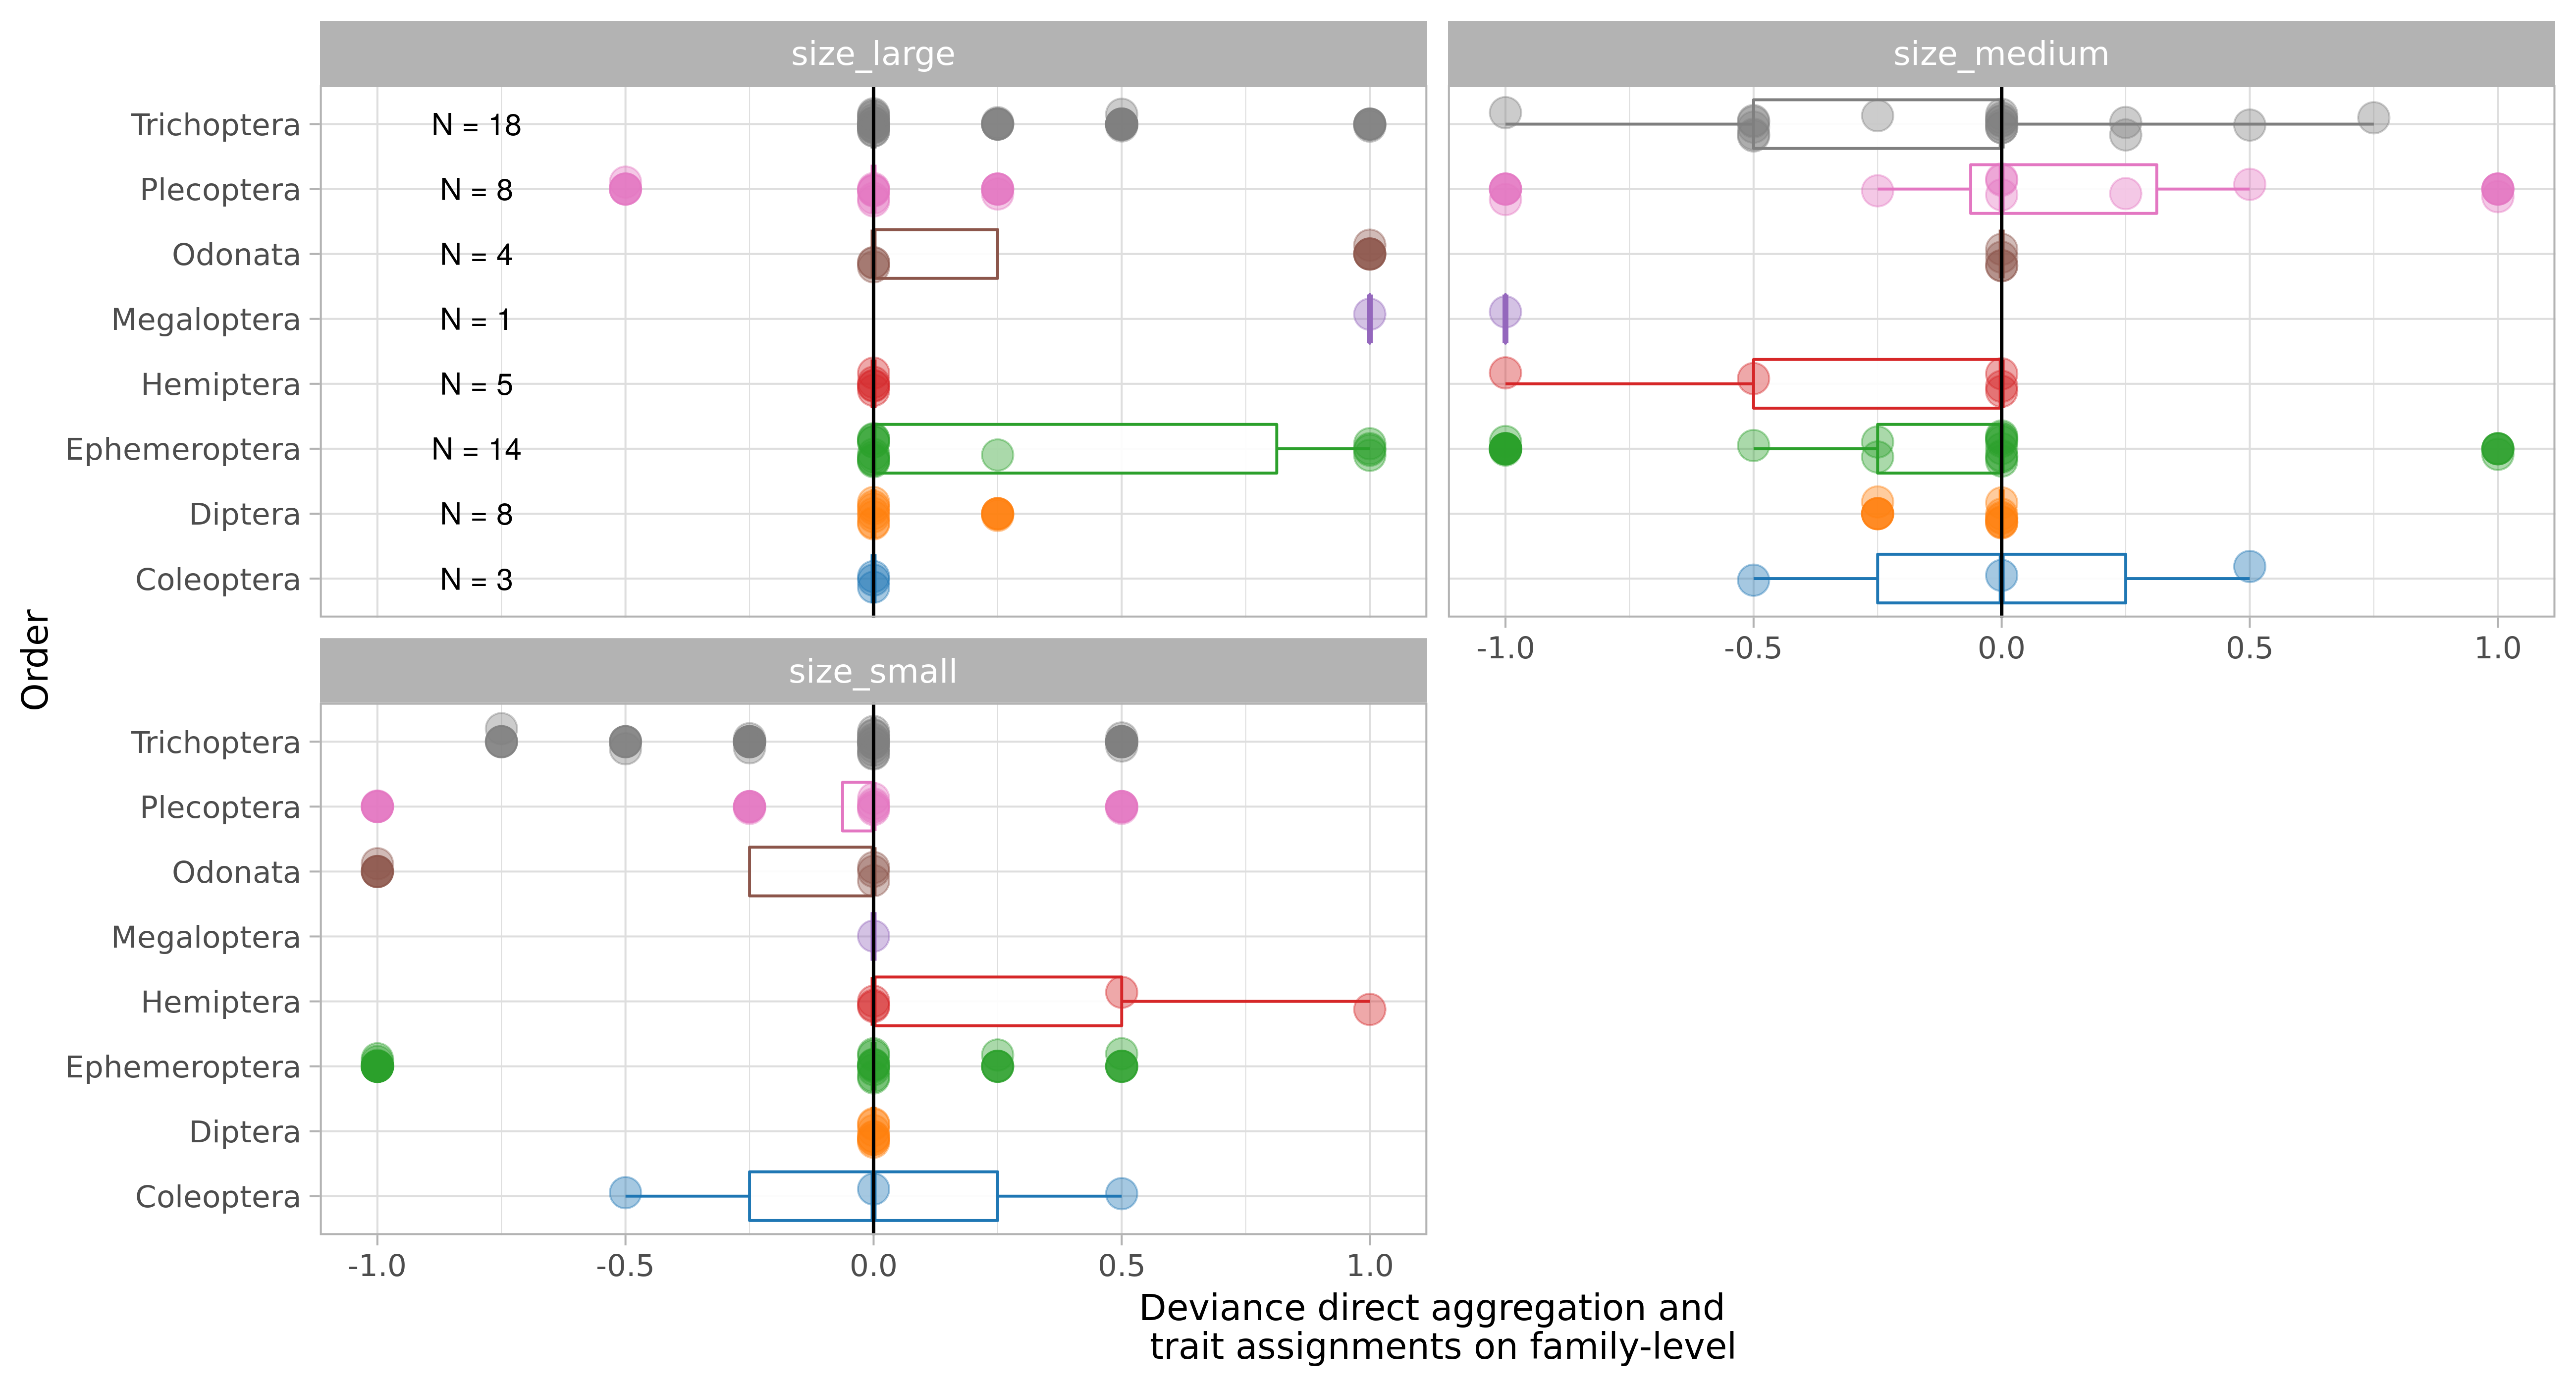
\includegraphics[width=14cm, height=7.5cm]{trait_deviations_dir_famlvl_size.png}
\end{figure}

\begin{figure}[H]
  \centering
  \caption{.}
  \label{fig:trait_dev_stepwise_agg_volt}
  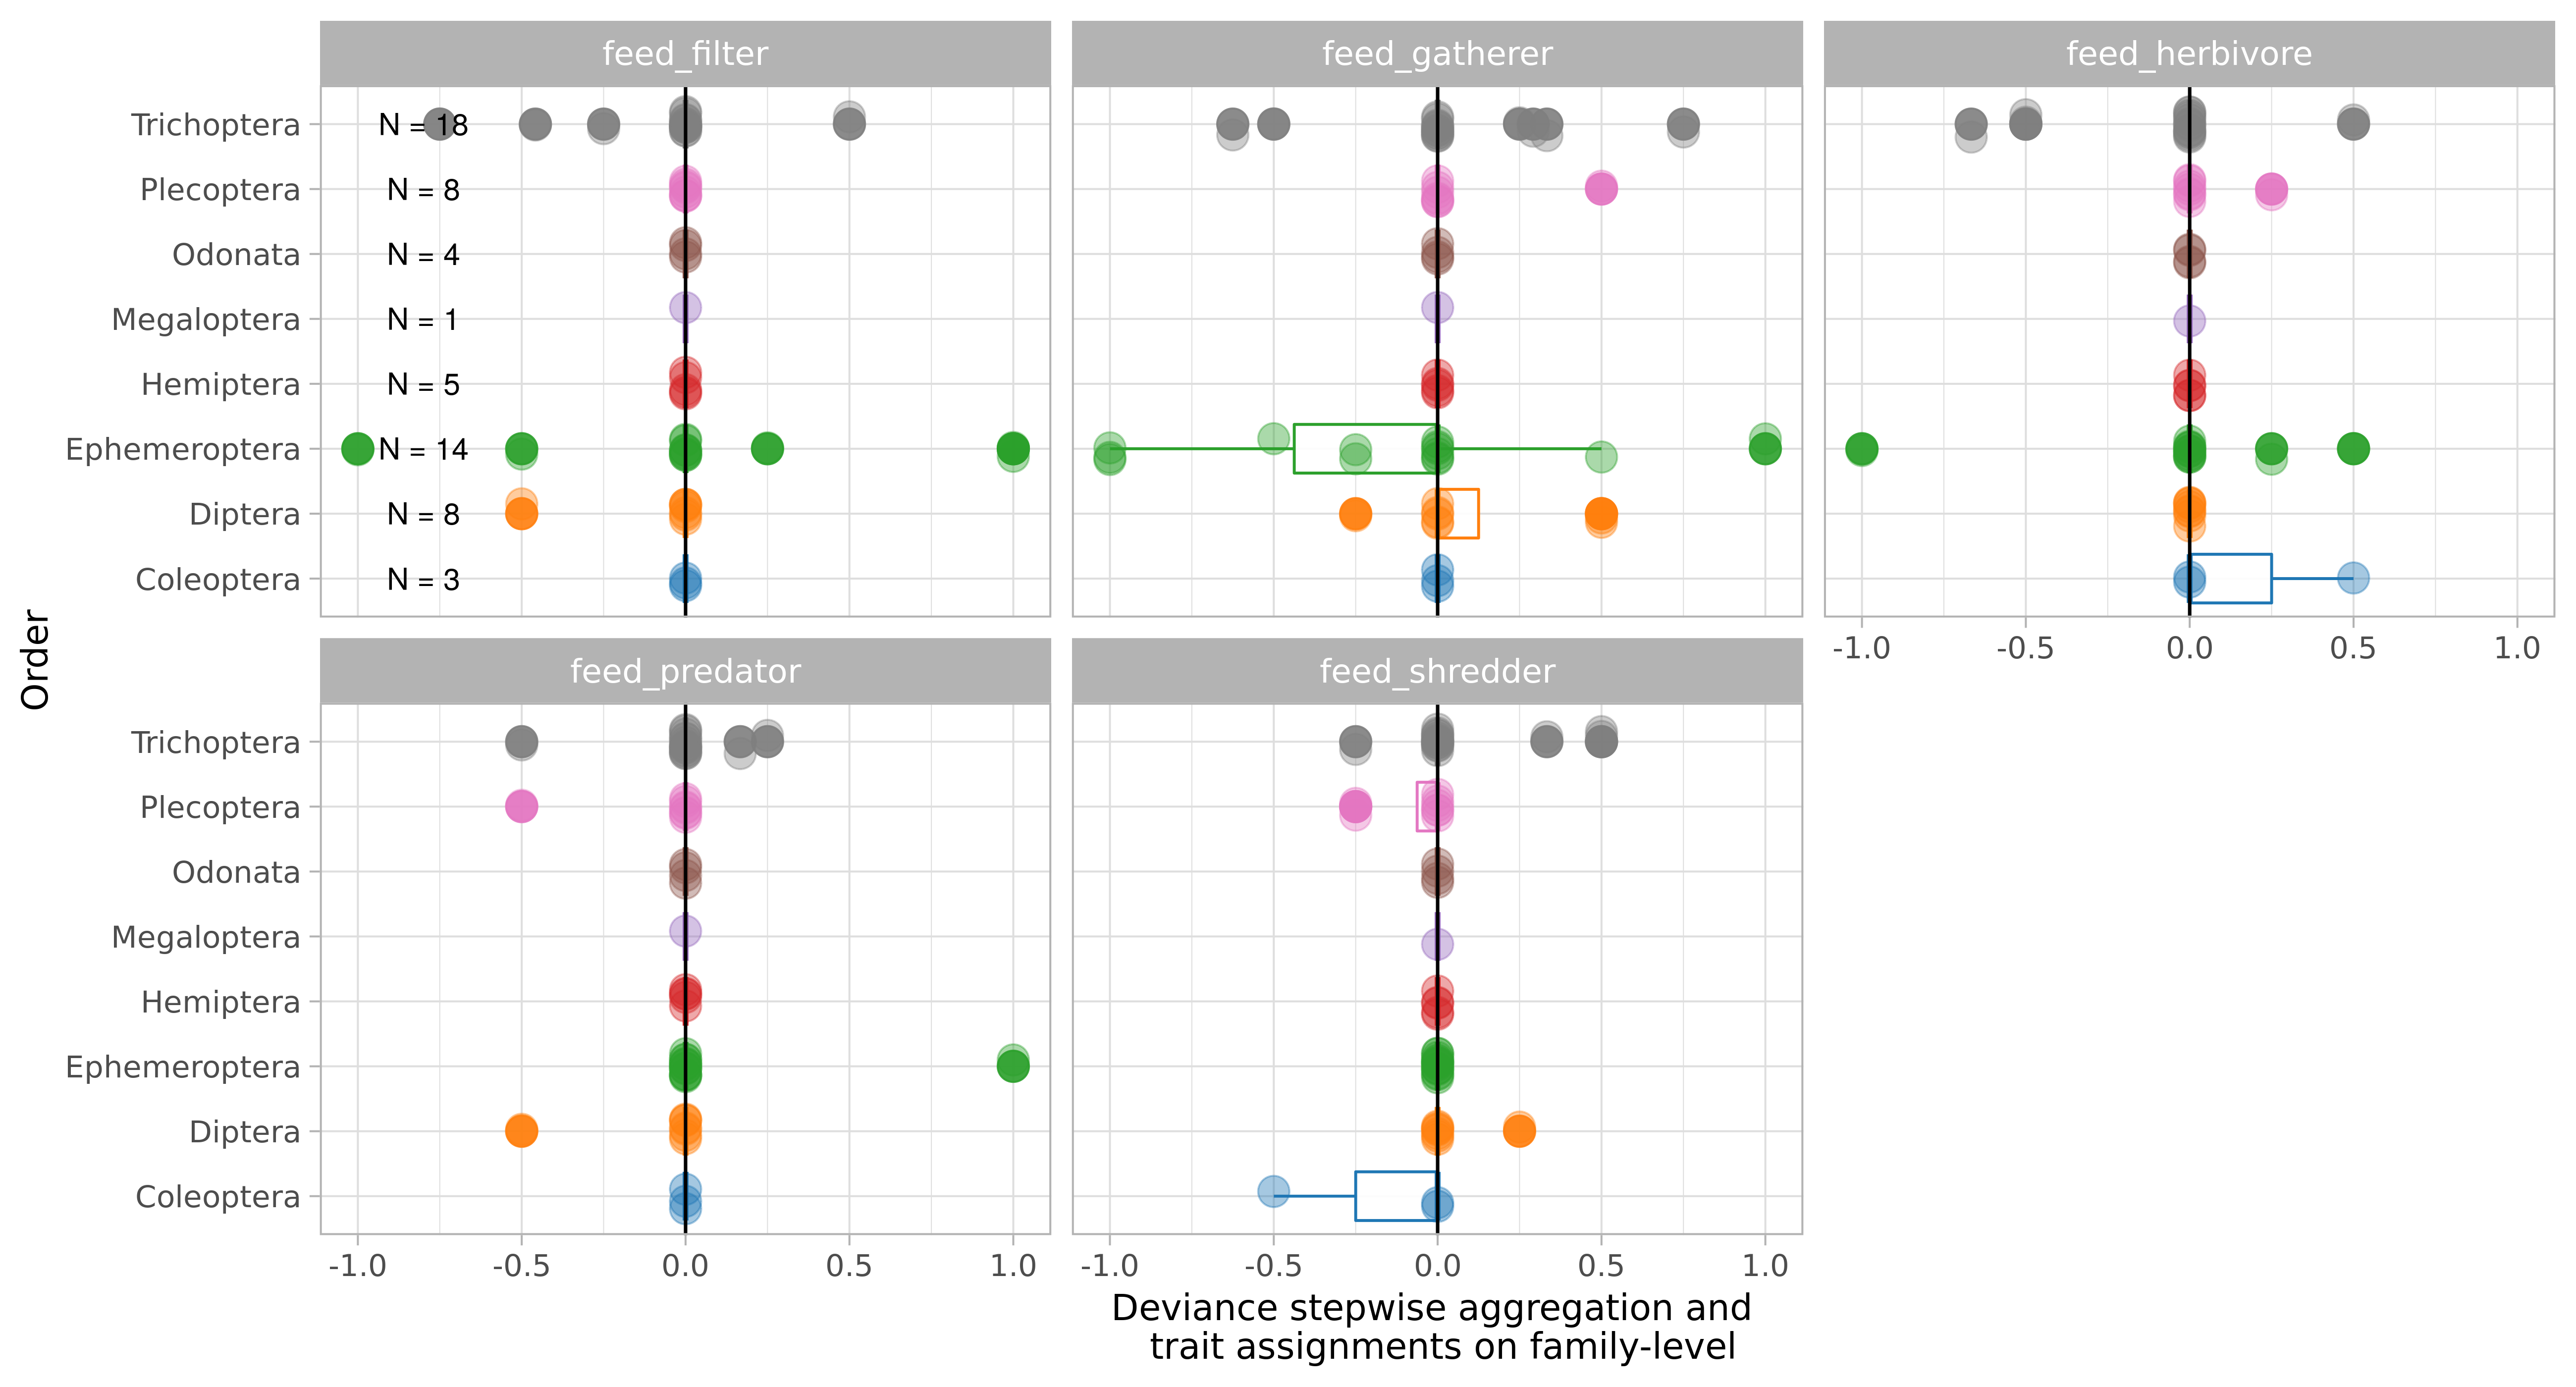
\includegraphics[width=14cm, height=7.5cm]{trait_deviations_stepwise_famlvl_feed.png}
\end{figure}

\begin{figure}[H]
  \centering
  \caption{.}
  \label{fig:trait_dev_stepwise_agg_locom}
  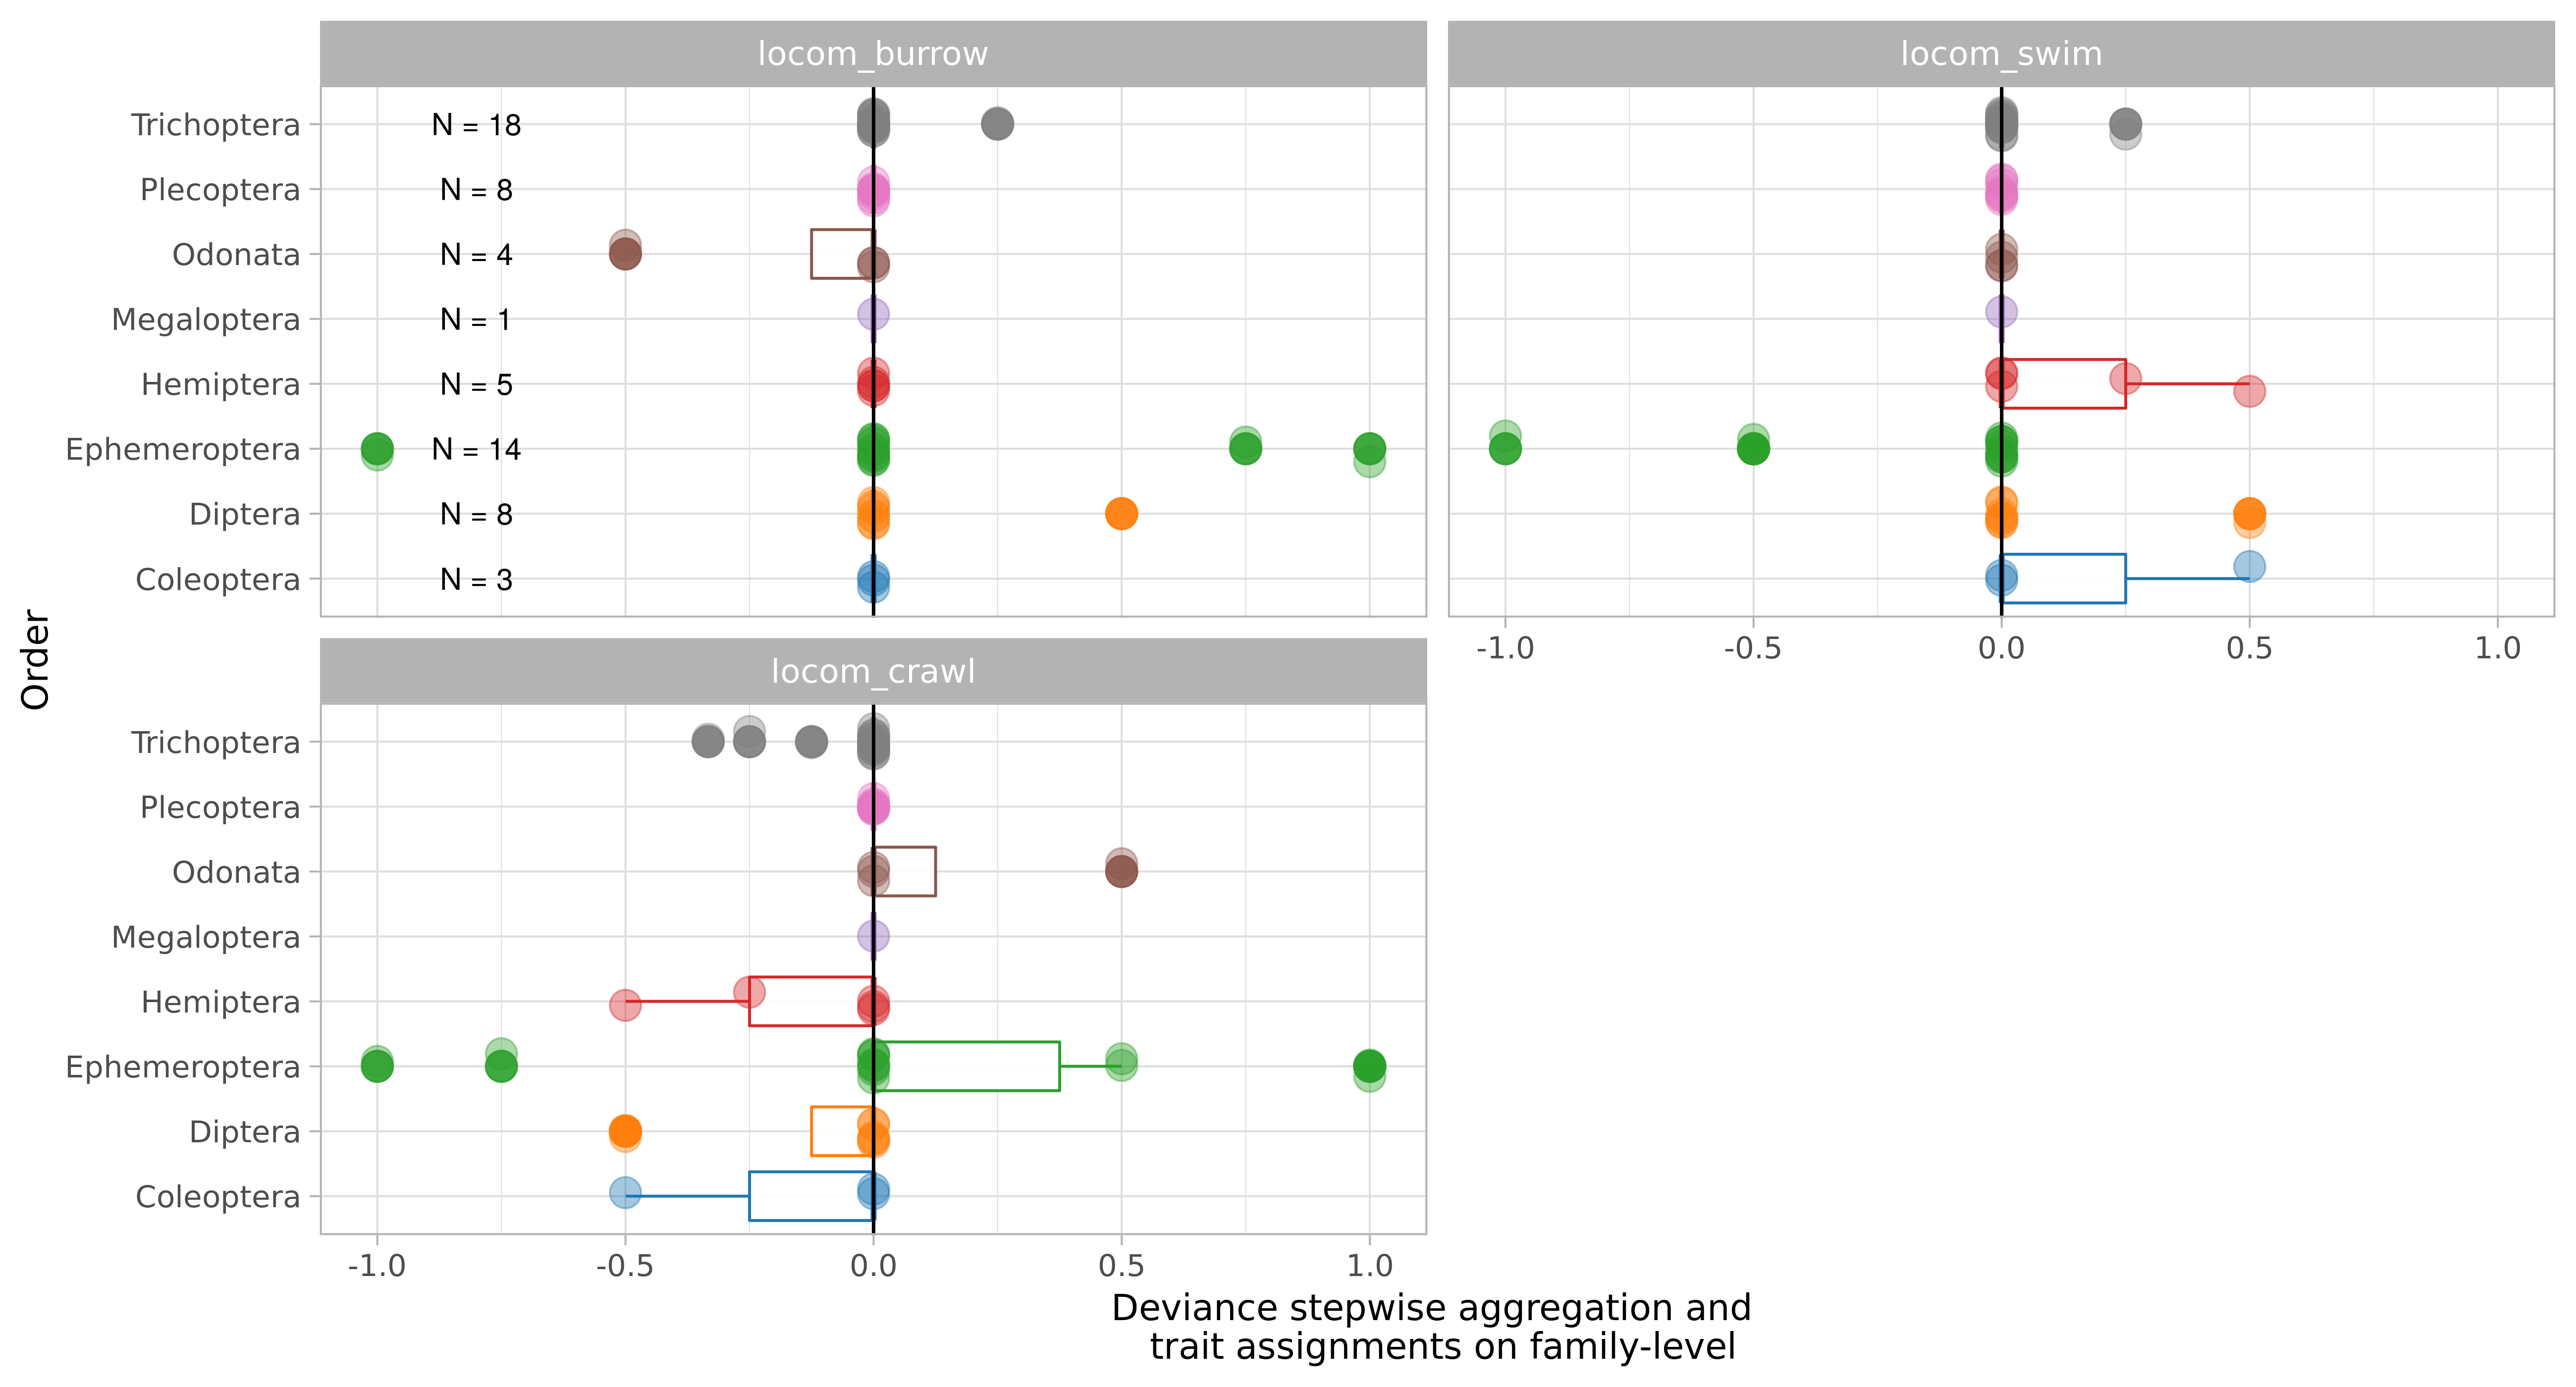
\includegraphics[width=14cm, height=7.5cm]{trait_deviations_stepwise_famlvl_locom.png}
\end{figure}

\begin{figure}[H]
  \centering
  \caption{.}
  \label{fig:trait_dev_stepwise_agg_resp}
  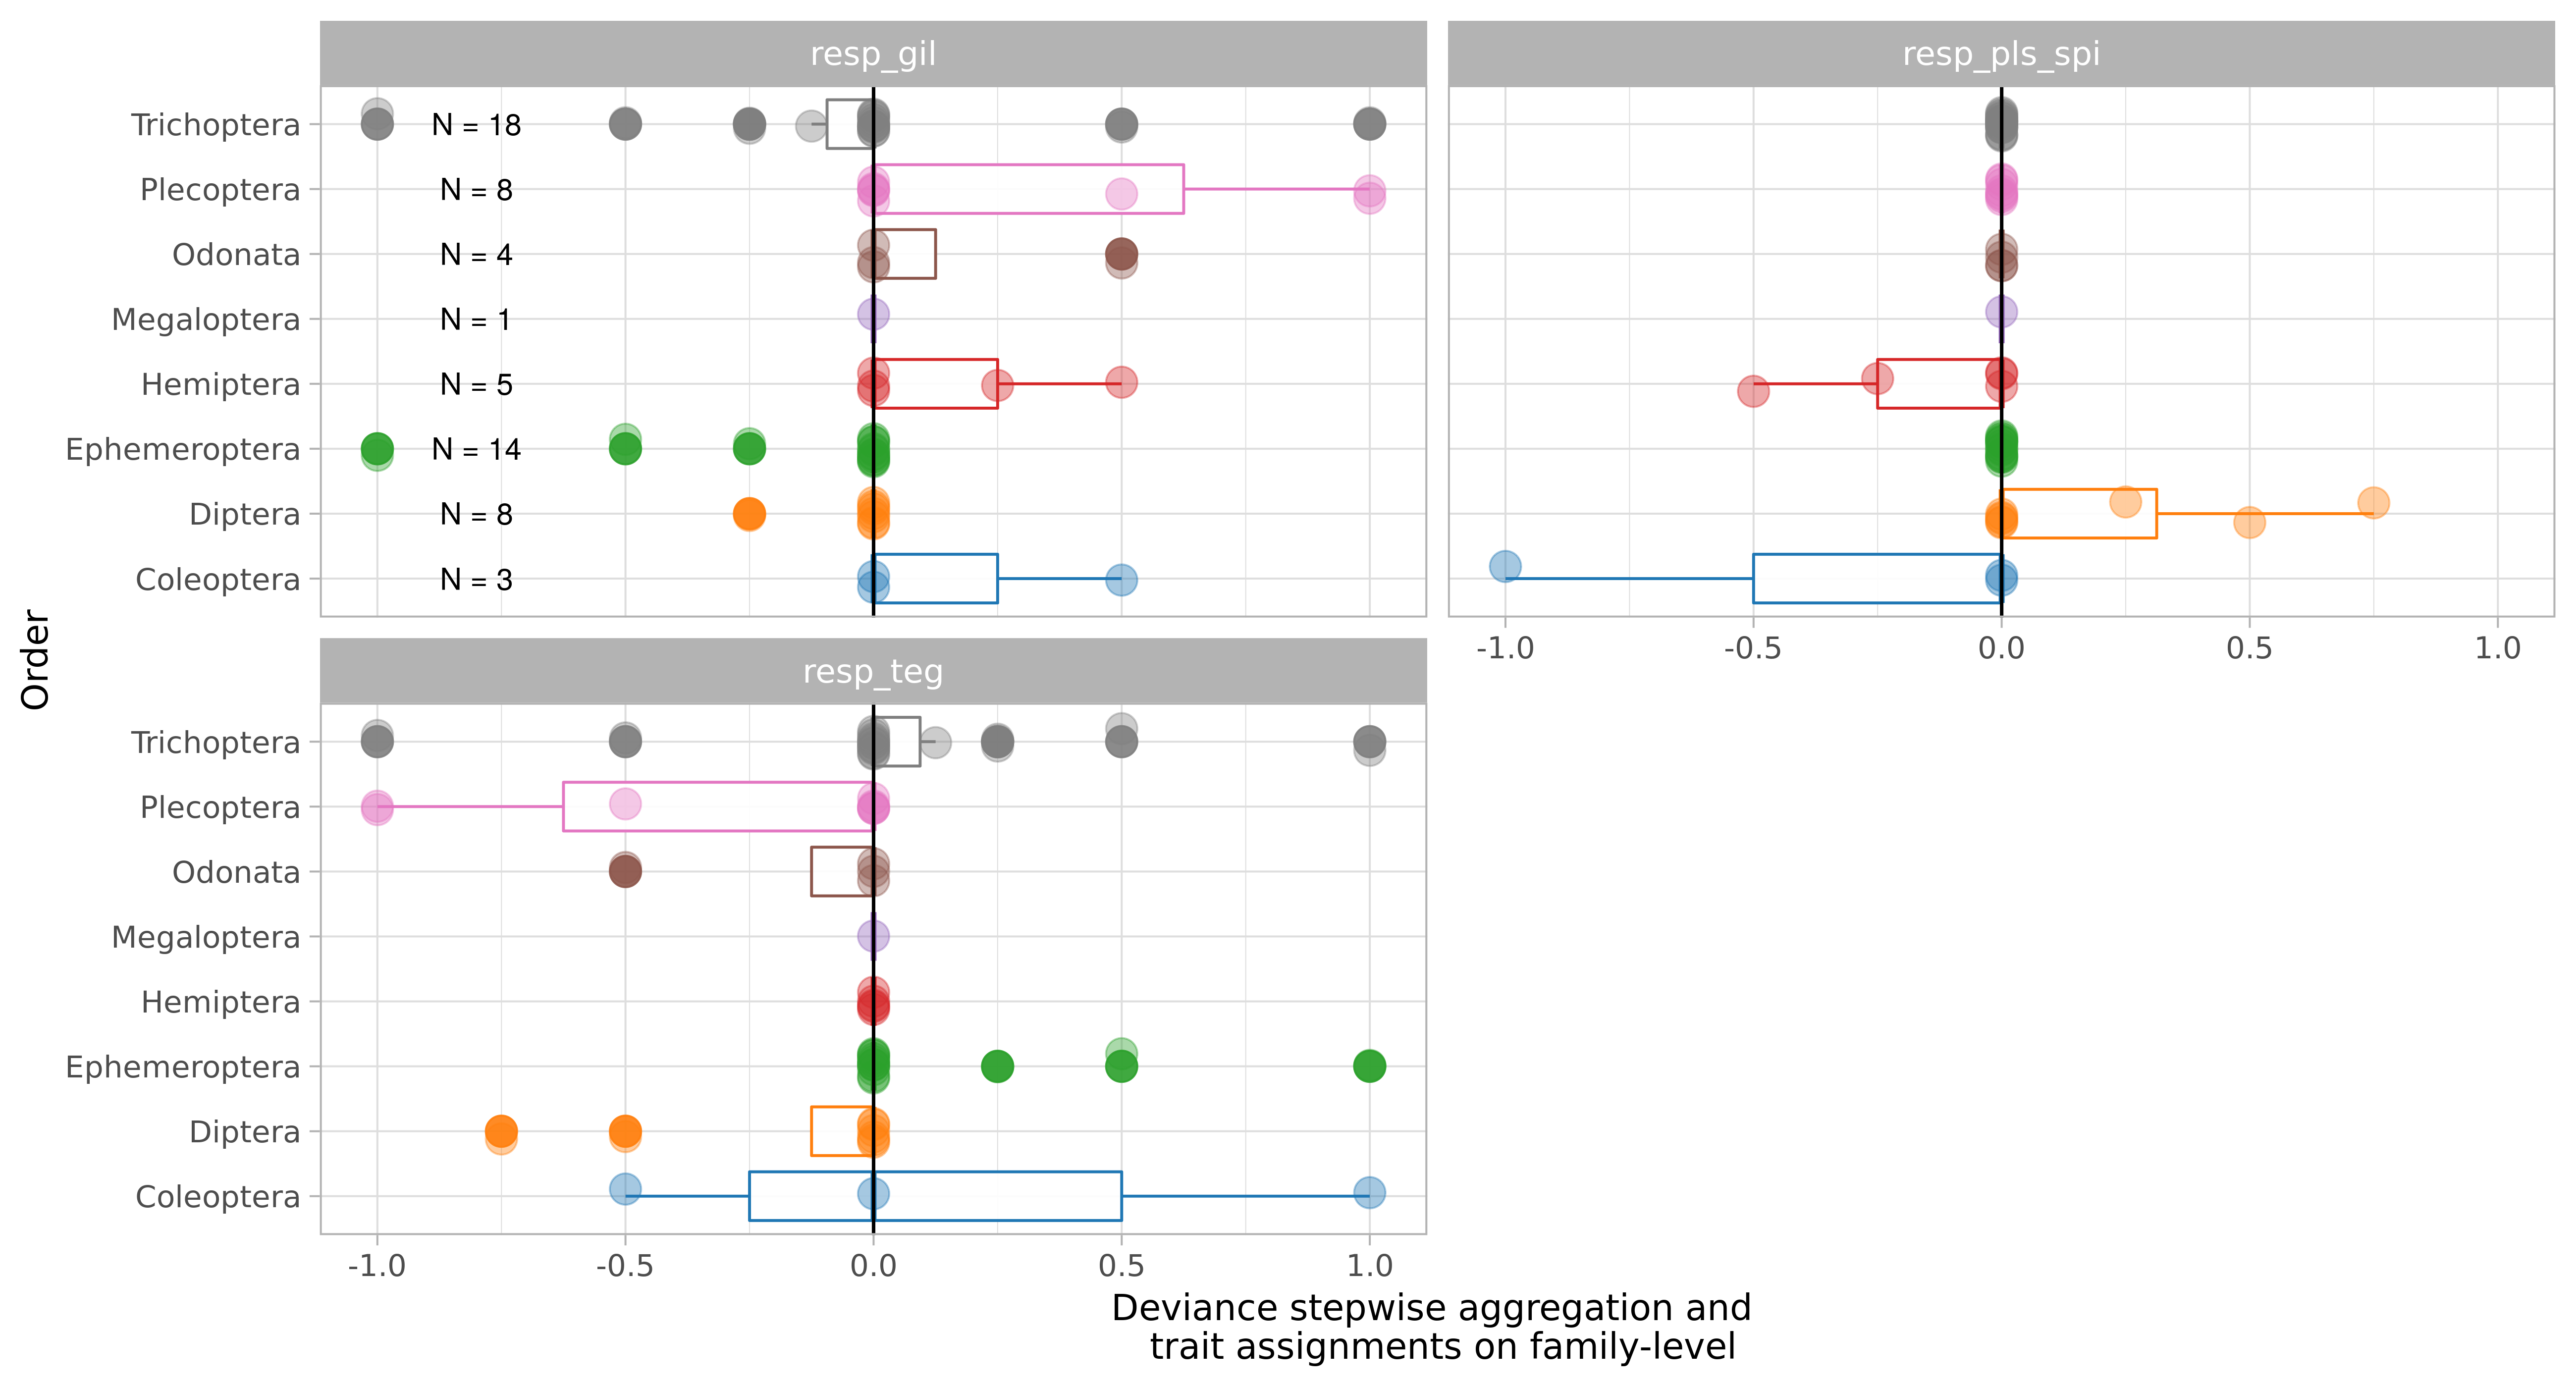
\includegraphics[width=14cm, height=7.5cm]{trait_deviations_stepwise_famlvl_resp.png}
\end{figure}

\begin{figure}[H]
  \centering
  \caption{.}
  \label{fig:trait_dev_stepwise_agg_size}
  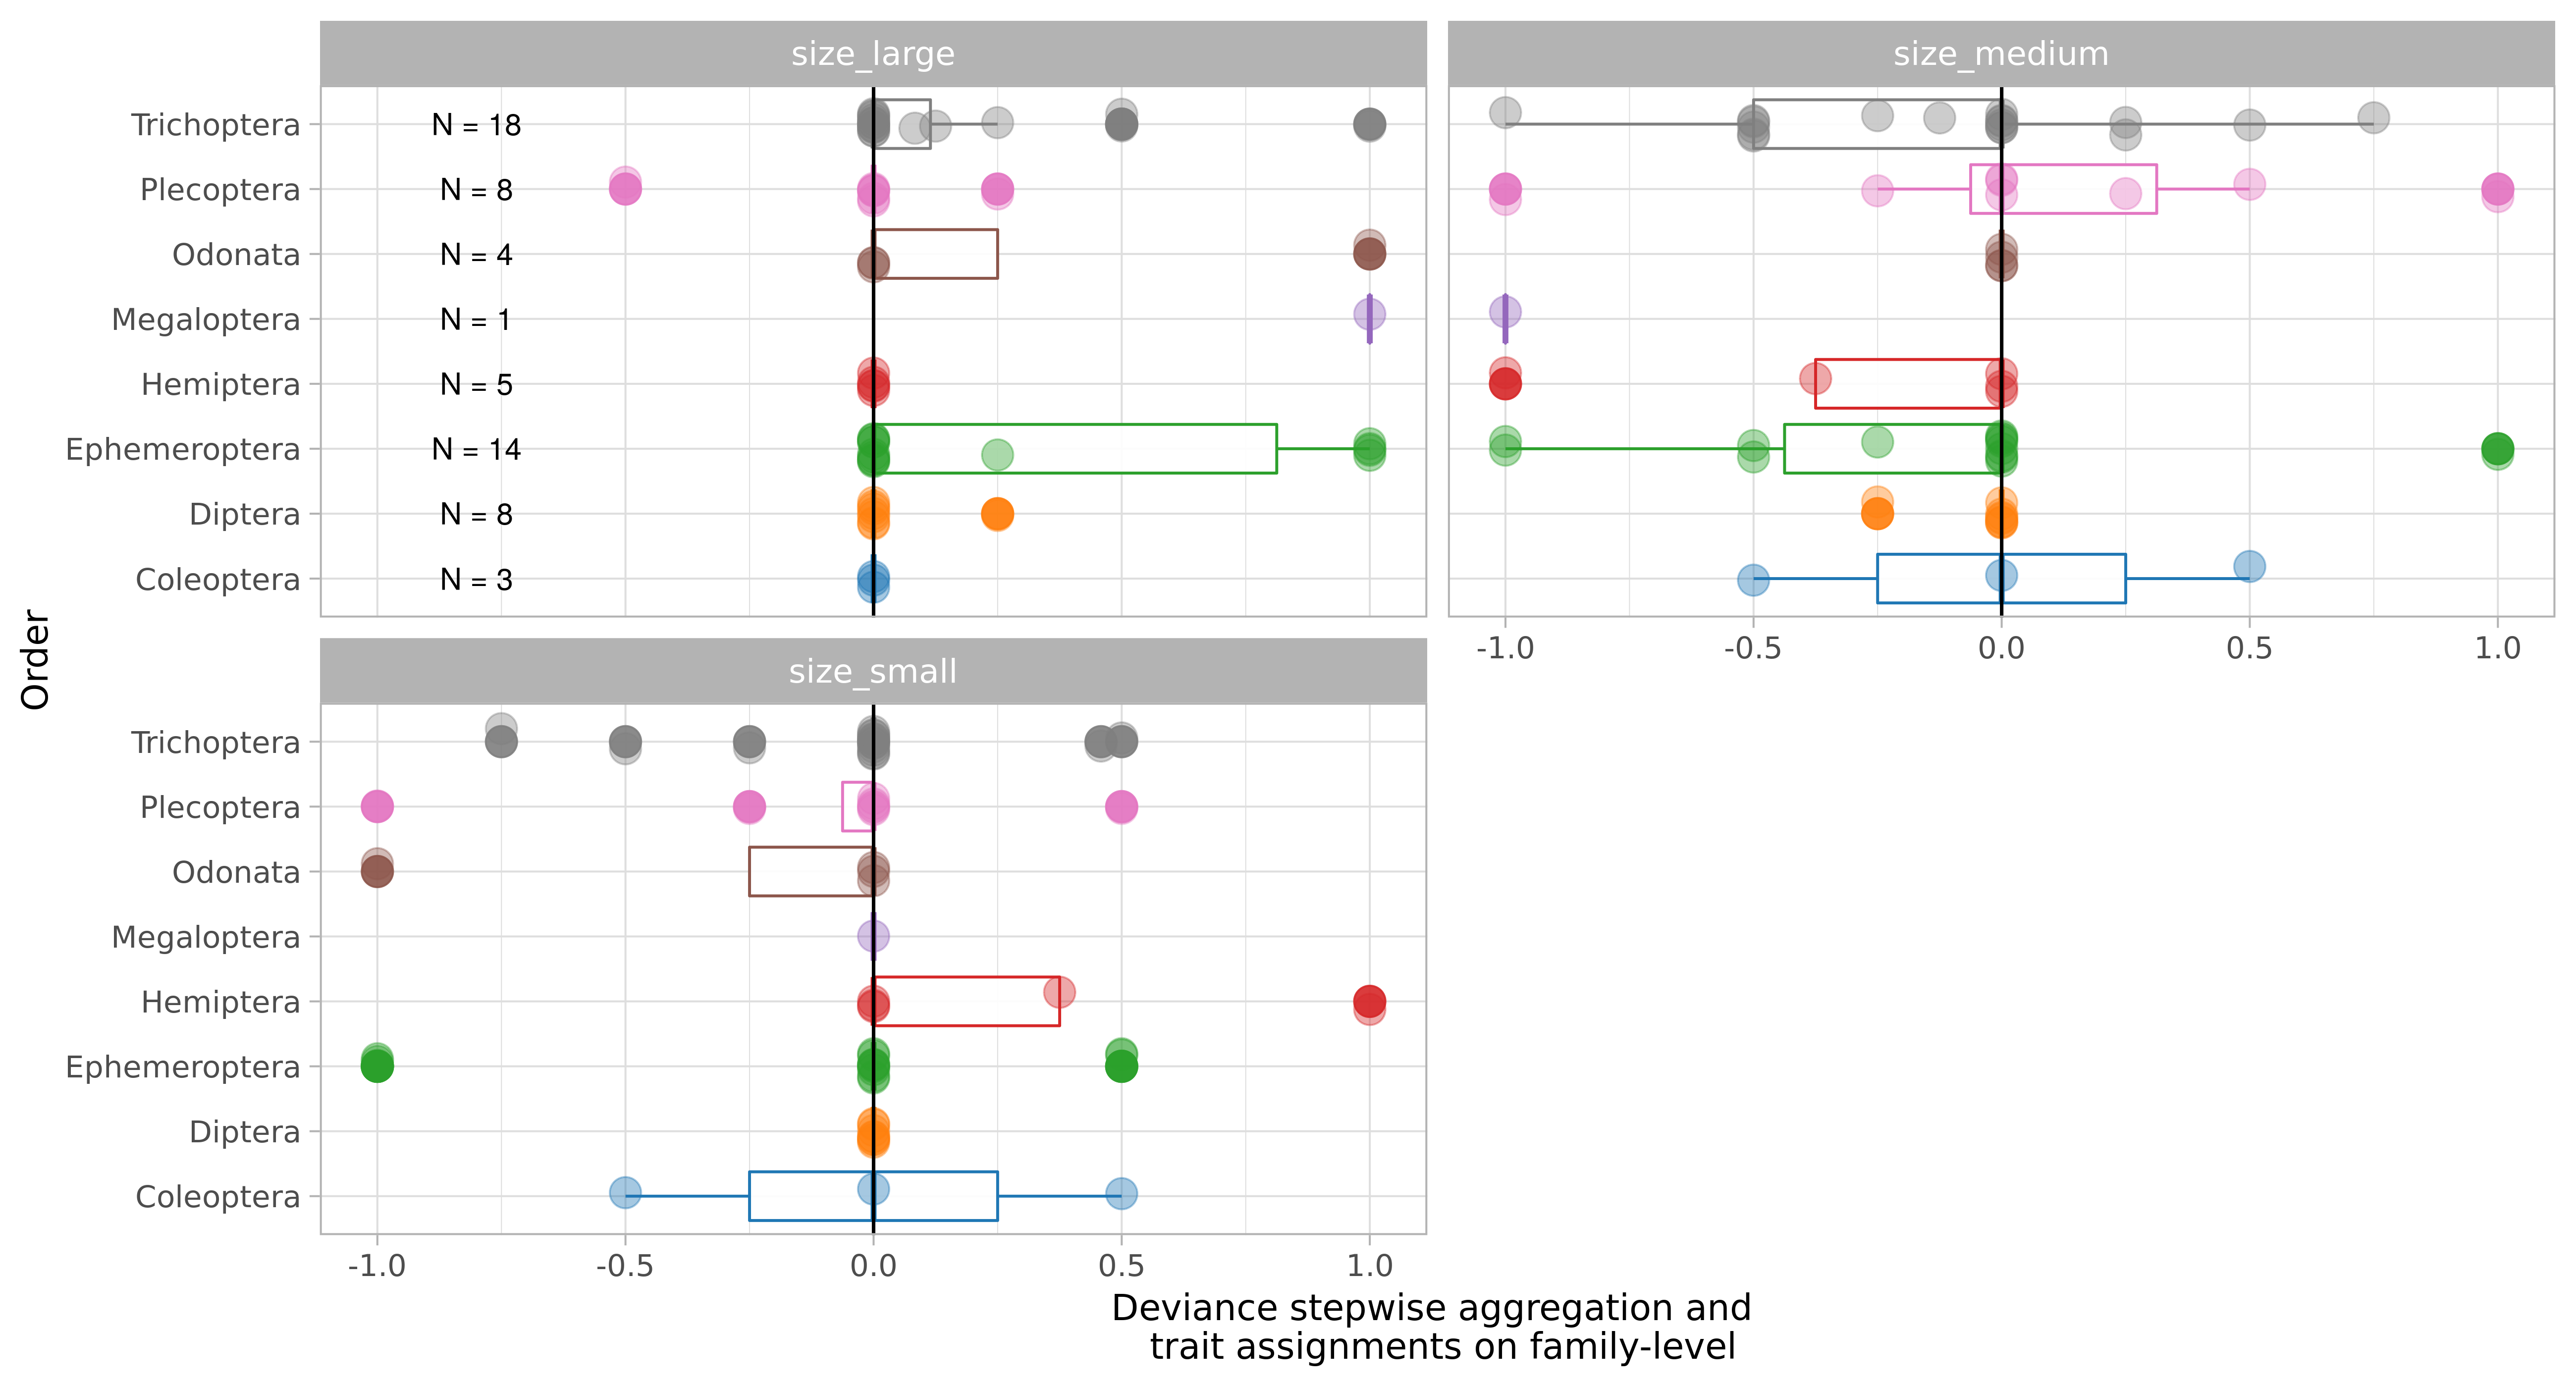
\includegraphics[width=14cm, height=7.5cm]{trait_deviations_stepwise_famlvl_size.png}
\end{figure}

\begin{figure}[H]
  \centering
  \caption{.}
  \label{fig:trait_dev_stepwise_agg_volt}
  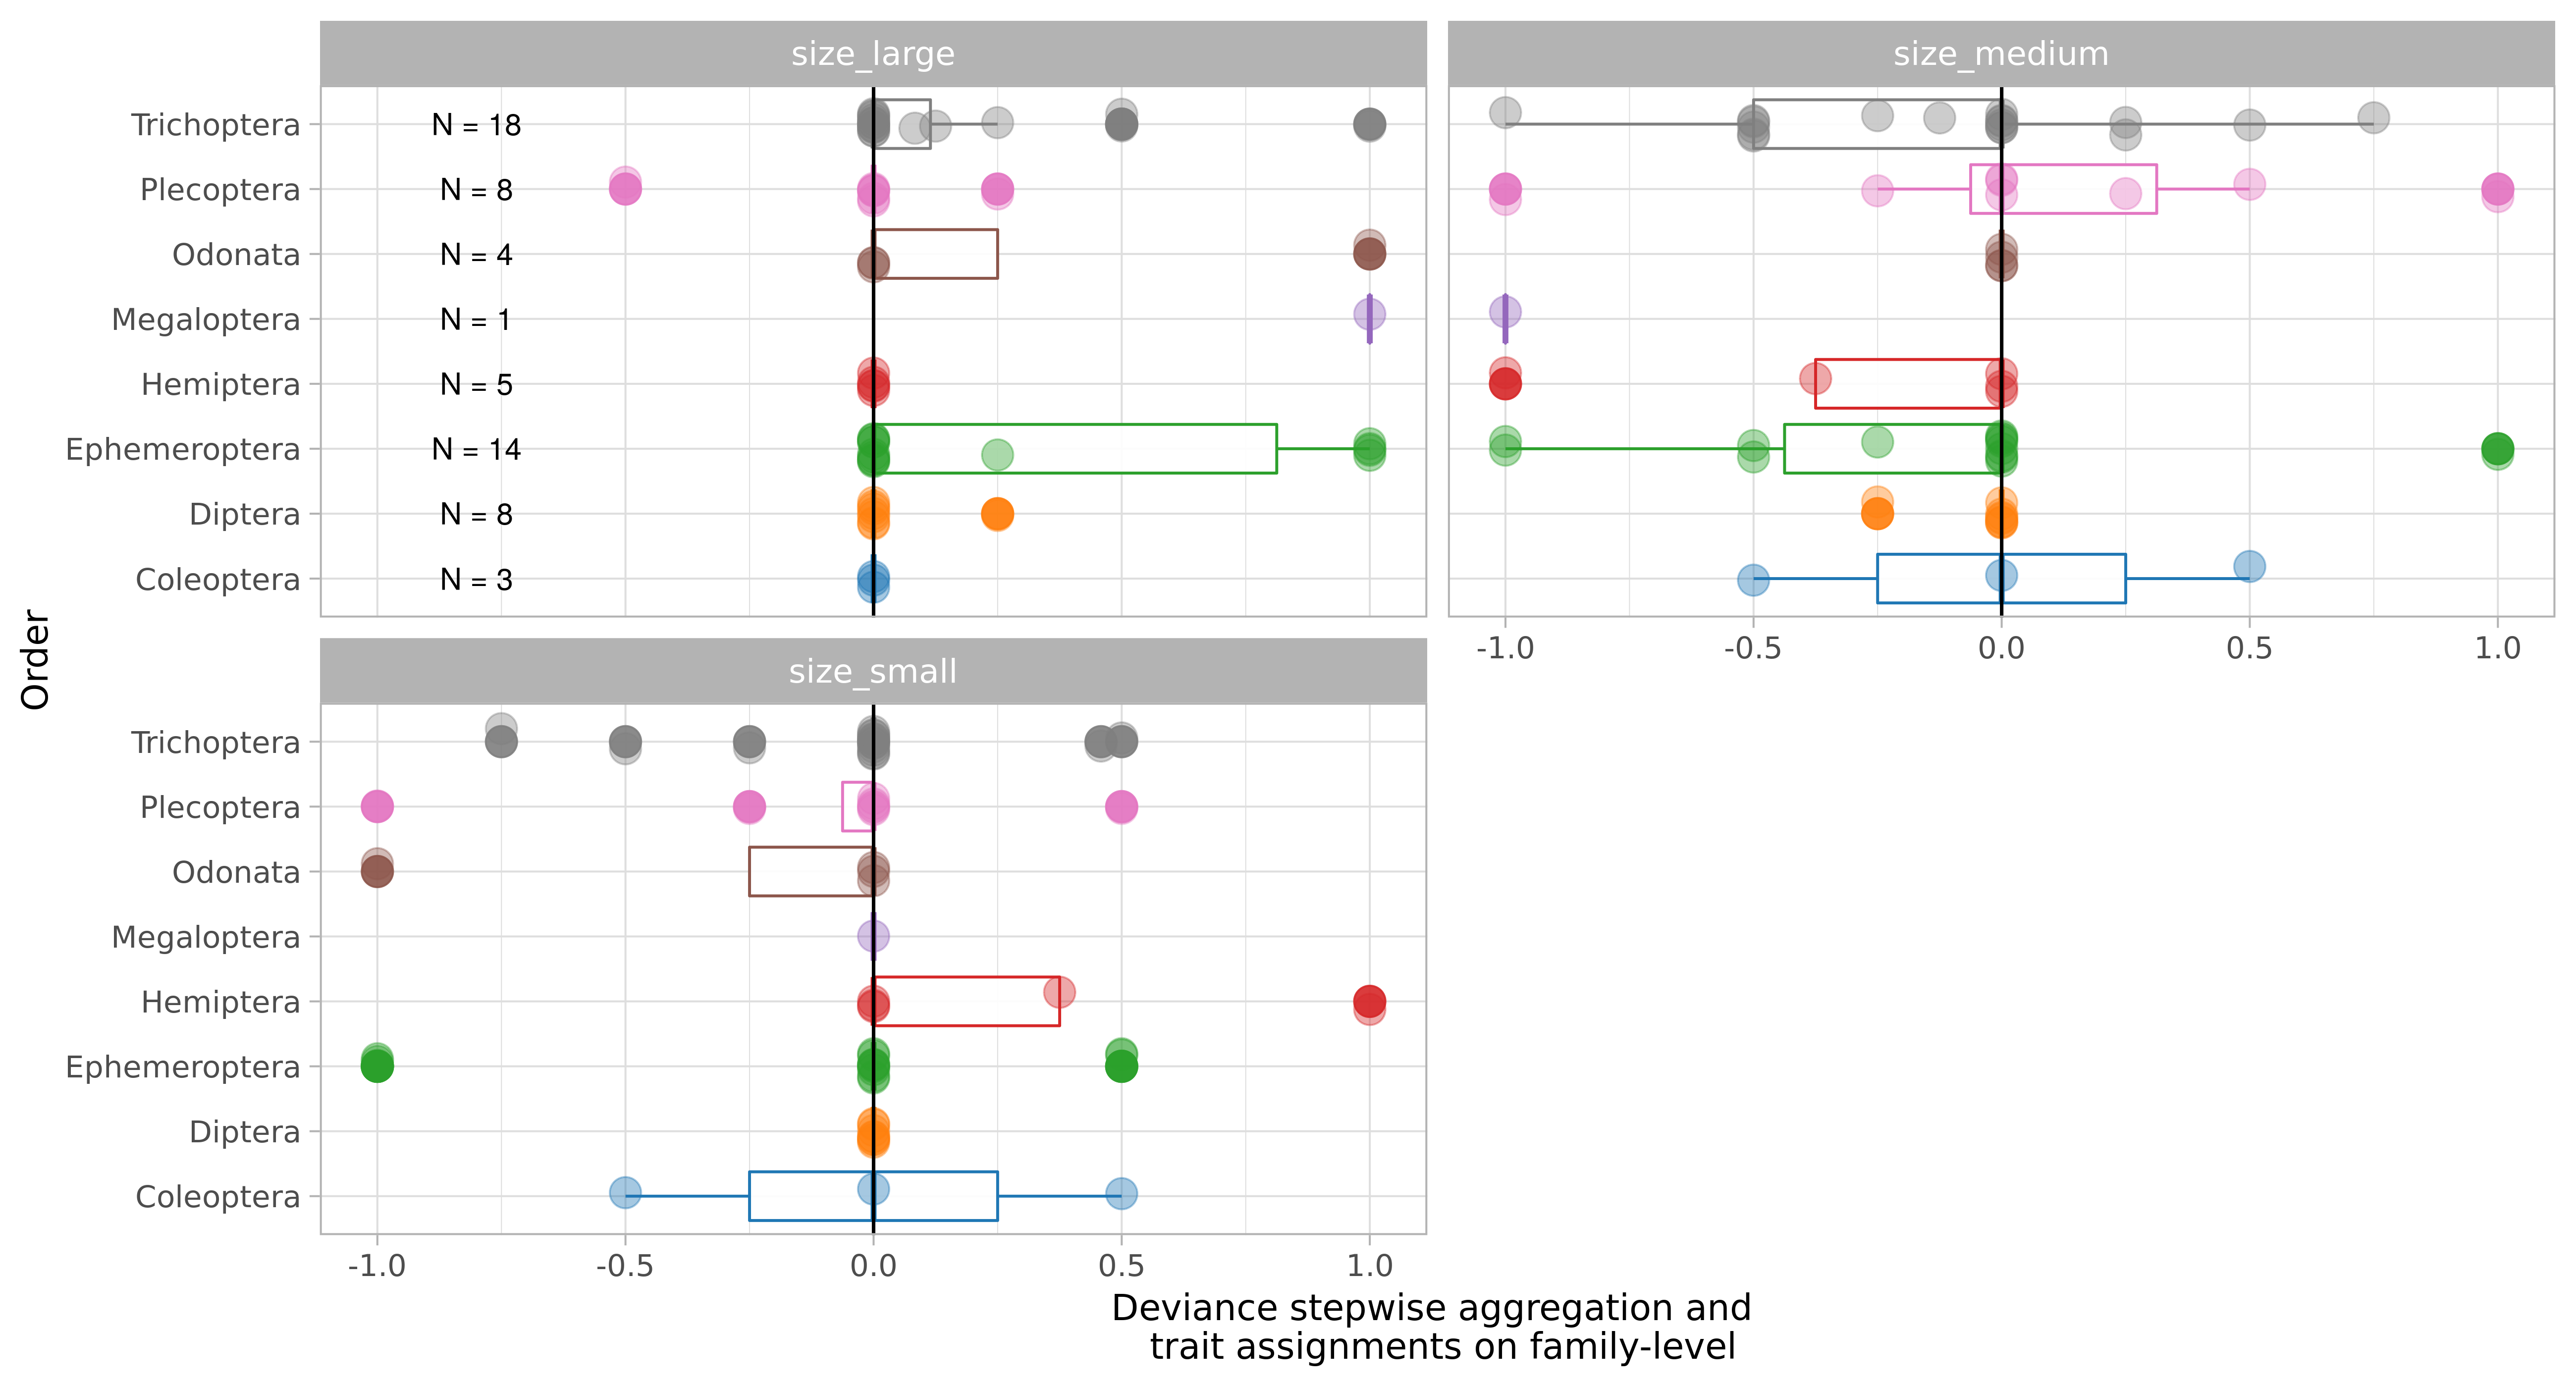
\includegraphics[width=14cm, height=7.5cm]{trait_deviations_stepwise_famlvl_size.png}
\end{figure}

%%%%%%%%%%%%%%%%%%%% \section*{Additional ideas} %%%%%%%%%%%%%%%%%%%%

% Section Description of databases:
% \begin{itemize}
%     \item Describe different databases briefly?
%     \item State goal of analysis $\rightarrow$ reference to second paper?
% \end{itemize}

\end{document}